\documentclass[12pt]{article}
\usepackage{times}
\usepackage{graphicx}
\usepackage{cite}
\usepackage[margin=1in]{geometry}
\usepackage{bm}
\usepackage{cleveref}
\usepackage[font=small,labelfont=bf]{caption}
\usepackage{subcaption}
\captionsetup[subfigure]{subrefformat=simple,labelformat=simple}
\renewcommand\thesubfigure{(\alph{subfigure})}
\geometry{a4paper}
\usepackage{float}
%\usepackage{cite}
\newcommand{\beginsupplement}{%
  \setcounter{table}{0}
  \renewcommand{\thetable}{S\arabic{table}}%
  \setcounter{figure}{0}
  \renewcommand{\thefigure}{S\arabic{figure}}%
}
\usepackage{array}
\newcolumntype{L}[1]{>{\raggedright\let\newline\\\arraybackslash\hspace{0pt}}m{#1}}
\newcolumntype{C}[1]{>{\centering\let\newline\\\arraybackslash\hspace{0pt}}m{#1}}
\newcolumntype{R}[1]{>{\raggedleft\let\newline\\\arraybackslash\hspace{0pt}}m{#1}}

\begin{document}

\title{A Versatile Method for Simulating the Dynamic Mechanical Structure of F-Actin Networks}
% \title{Dynamics and Structure Formation of Active F-Actin Networks}
\author{Simon L. Freedman, Shiladitya Banerjee, Glen M. Hocky, Aaron R. Dinner}
\date{}
\maketitle
\begin{abstract}
  The cooperative mechanics of filamentous actin and myosin in the cytoskeleton comprise one of three active polymer
  networks that give the cell its shape, size, and motion. We have developed a computational model to study this network that incorporates 
  the mechanical interactions of actin filaments, actin crosslinkers, and myosin motors to further
  probe their behavior in a disordered ensemble, such as in vitro reconstitutions that mimic the cytoskeleton of non-muscle cells. 
  We benchmark this model against well established experimental results regarding fluctuations of
  semiflexible polymers, rheology of crosslinked actin networks, and actomyosin interactivity in sliding filament assays. 
  We use the model to show how we can reproduce, tune, and characterize important force propagating structures 
  recently been observed in experiment. 
\end{abstract}
\section{Introduction} 
The collective activity of many-particle systems where pair-wise particle interactions are well understood 
can be eluicidated via molecular dynamics simulations. 
A biomolecular example involves the proteins actin and myosin in the cytoskeleton of non-muscle cells. In that
environment, actin monomers polymerize into polar actin filaments (F-actin) which are microns long and
nanometers thick, and myosin motor proteins aggregate onto $0.4\mu m$ long backbones to form myosin minifilaments \cite{niederman1975}. 
For precessive motors, such as myosin II, the binding of myosin to actin, followed by ATP hydrolosis and subsequent
unbinding, results in the relative motion of myosin with
respect to actin toward the positive (barbed) end of an actin filament. In the cytoskeleton, this
motion drives many biological processes, including endocytosis, cell-division and maintenance of cell shape
\cite{stricker2010, murrell2012}.
\par
The mechanism through which myosin can walk on actin has been extensively studied in muscle cells, where actin
filaments are arranged in parallel bundles called sarcomeres. A myosin filament binds to two antipolar
sarcomeres, walks toward the barbed end of both, and the tension along the myosin pulls the 
sarcomeres together, resulting in muscle contraction\cite{huxley1969}. 
However, in the cytoskeleton of nonmuscle cells, there is no inherent ordering of actin or myosin filaments, so while
interactions between individual myosin and actin filaments exist, how 
they act in concert to produce a variety of behaviors is an active area of research \cite{murrell2012, stam2015, murrell2015}. 
\par
Recent experimental studies \cite{murrell2012, murrell2014} have reconstituted networks of
actin and myosin, and analyzed how changing their respective concentrations, lengths, elastic properties, and binding affinities
can effect the ability of a disordered ensemble to contract and form static structures. They have also incorporated
various actin binding proteins (crosslinkers) into their experiments such as filamin, scruin, and $\alpha$-actinin, as these are
instrumental in crosslinking actin filaments to form long lasting, force propogating bundles and networks
\cite{gardel2004, murrell2012, murrell2014, murrell2015}. 
The goal of these experiments is ultimately to develop a phase diagram that shows the importance of 
key players of active networks, such as myosin density \cite{murrell2012}, actin bundle rigidity \cite{murrell2012},
and cross-linker density\cite{murrell2014} in structure formation and force generation within the cytoskeleton.  
\par
For example, by varying the density of myosin added to a reconsituted actin network, one can vastly effect its biomechanical
behavior. At low
motor density, the myosin will translocate large distances but will not cause the network to contract\cite{burov2013}. Above a
critical density, the myosin will contract the network and raising the density further will result in more extensive
contraction. However, there also appears to exist a second critical density past which more motors are ineffective 
at increasing contractility \cite{murrell2014}. These in vitro experiments have also been used to probe the underlying
mechanisms that control the ensemble network behavior. 
Key mechanistic results indicate that actin filament buckling and severing as well as relative actin and myosin sliding
are all necessary for network contraction \cite{murrell2012, murrell2014}.
\par
The goal of this work is to present a mathematical model, in the form of a non-equilibrium molecular dynamics
simulation, that can efficiently explore the phase space of this actin, myosin, and crosslinker system.  
This mathematical model can guide our understanding of the relationship between
the microscopic biochemical protein-protein interactions and the macroscopic mechanical functionality of the ensemble. Additionally,
because the model simulates actin, myosin, and crosslinkers in space and time, it will enable us to learn the trajectory
of an ensemble, and how intermediate mesoscopic structures tune network functionality.
\par
The key achievements of this model are that it is well bench-marked to reproduce known experimental results for actin
filaments, ensembles of actin and crosslinkers (passive networks), and ensembles of actin and myosin 
(active networks). 
At the polymer level, we will reproduce predicted spatio-temporal fluctuations of actin filaments. 
For passive crosslinked networks we will reproduce known stress strain
relationships. For active networks, we will reproduce well-understood velocity distributions of actin
filaments in a myosin motility assay. We will then use the simulation to demonstrate how ensembles of randomly oriented
actin filaments and crosslinkers can be rearranged by myosin motors to form tunable structures with distinct biophysical and
mechanical functionality.  
\par
While our simulation is motivated by in vitro experiments, the setup has been influenced by several other computational
models of actin and myosin. We briefly review these various computational models to show how other models have
influenced ours, and where we differ.
Most prominently, a number of publications have dealt with understanding the rheological properties of crosslinked actin
networks\cite{mackintosh1995, head2003, wilhelm2003, kim2009}.  
For example, to study the viscoelasticity of passive networks,  Head, et al., simulated distributed actin filaments randomly 
on a $2D$ plane, added cross-links at all intersections of the filaments to form a network, sheared 
this network and let it relax to a minimum energy, corresponding to a chemical equilibrium \cite{head2003}. 
From this model, they were able to identify three elastic regimes,
characterized by the mean distance between crosslinkers and the temperature. 
Dasanyake, et. al., extended this model to include a term in the potential energy that corresponded to
myosin motor activity, and observed the emergence of force chains that tramsmit stress throughout the network,
which could help understand how contractile stress can emerge from a disordered network \cite{dasanyake2011}.
These models predict the mechanical equilibrium behavior of the actin / cross-linker and the actin / myosin
systems; i.e., at a particular time, they answer questions such as, how well can this cytoskeletal network propogate
force, and how can crosslinker concentrations alter mesh stiffness.
\par
Other simulations focus on the ensemble motion of a myosin minifilament with respect to a single actin filament.  
Erdmann and Schwarz used Monte Carlo simulations to verify a master equation that expresses the probability that $N$ motors are 
bound at time $t$ to a single filament\cite{erdmann2012}. Based on this model they are able to make accurate predictions for 
the duty ratio and force velocity curves for myosin. Stam et al. used simulations to study force buildup on a single 
filament by a multi-headed motor and found
distinct timescale regimes over which different biological motors could exert force and act as cross-linkers
\cite{stam2015}. These models of actin-myosin interaction are important to understand the mechanics at
the level of a single filament, and their results can be incorporated into larger network simulations. 
\par
Wang and Wolynes \cite{wang2012} model the F-actin networks as a graph of crosslinkers (nodes) and rigid actin filaments
(edges) in which myosin motor activity is simulated via antisymmetric kicks along the filaments. Their results include a
binary phase diagram of networks which are either contractile or not as a function of cross linker and myosin
densities. While the simplicity of their model is intriguing, their simulation does not account for filament bending, 
and their integration is performed via Monte Carlo, and is thus more applicable to structure formation than dynamics.
Nedelec performs dynamic simulations of ensembles of semiflexible microtubules and kinesin motor proteins
which have many of the same properties as actomyosin networks and uses them to explore aster and network formation in microtubule
assays \cite{nedelec2007} and has recently shown their applicability to actin networks \cite{ennomani2016}.
Gordon et al. \cite{gordon2012} and Kim \cite{kim2014} similarly simulate dynamics of F-actin networks and include
semiflexible filaments, motors and cross linking proteins. Gordon succeeded in showing various structures that can emerge
from assemblies of this type and Kim shows how changing concentrations of cross linker and motor densities can alter how
much force is generated by the network.
\par
Our model is constructed by including many of the best features of these preceding models.
We will use the potential energy for an actin filament as described by Head et al., for simulating actin filaments that can 
both bend and stretch, and also initialize our networks similarly, by placing cross-linkers initially at intersections 
to form well connected networks. In contrast to references \cite{head2003, dasanyake2011}, we will 
simulate non-equilibrium dynamics, including fluctuations due to non-zero temperature,  
cross-linkers and myosins binding and unbinding, and the precessive activity of myosin.  
We will use predictions from \cite{stam2015} to extrapolate numerical
parameters for the binding kinetics of a myosin mini-filament as they relate to a single myosin head and use this extrapolated
bulk behavior of a mini-filaments. Force propagation rules and binding kinetic equations will be similar to those of
\cite{nedelec2007, gordon2012} with slight differences in how we actually simulated the fluctuating filaments. 
Our simulations will be most similar to those performed in references \cite{kim2014, ennomani2016} and we hope to
expand on their methods of exploring actomyosin via agent based molecular dynamics by showing how they can shed light on 
a variety of systems of current experimental interest.
\section{Model}  
In the interest of computational efficiency we have chosen to coarse grain actin filaments, myosin minifilaments, and
crosslinker proteins at length scales relevant for network behavior. Actin filaments are
modeled as polar worm-like chains (WLC) such that one end of the WLC represents the barbed end of a filament and the
other end of the filament represents its pointed end. This implementation allows for filament sliding and filament
buckling, as seen in \Cref{fig:toys}, both of which are instrumental for actomyosin contractility \cite{murrell2012}. 
Cross-linkers are modeled as Hookean springs such
that both ends of the spring (heads) can bind and unbind from filaments. Model crosslinkers can therefore increase network connectivity
which is understood to increase the length-scale of network contraction \cite{murrell2015} and yields actin bundles
which are often seen in experiment \cite{gardel2004, murrell2012, murrell2014}. Myosin minifilaments are cross-linkers such
that a head is bound to a filament will walk toward the filament's barbed end. Thus they are able to slide filaments,
translocate across filaments, and increase network connectivity, which are instrumental mechanisms when determining
network behavior\cite{murrell2014}. We chose to parameterize our model in $2D$ as the in vitro experiments we wish to
interpret are relatively flat and
approximating the system as $2D$ allows us to simulate larger systems for longer times. Because we use a $2D$ system to
represent a $3D$ experiment, we do not include exclude volume for our filaments and crosslinkers, to account for
some of the freedom lost from the reduction in dimensionality.
\begin{figure}[H] 
  \centering
  \begin{subfigure}{0.95\textwidth}
    \centering
    \includegraphics[width=\textwidth]{figs/slide/t0t3t10_black.eps}
    \caption{\label{fig:slide}}
  \end{subfigure}
  \begin{subfigure}{0.95\textwidth}
    \centering
    \includegraphics[width=\textwidth]{figs/buckle/t0t3t10_black.eps}
    \caption{\label{fig:buckle}}
  \end{subfigure}
  \caption{%
  \label{fig:toys}%
  Time series of two antiparallel $10\mu m$ filaments (red) undergoing contraction via one motor (white) and one
  crosslinker (yellow). The barbed ends of each filament are marked by a blue dot. Left is $t = 0$, middle is $t = 3s$
  and right is $t = 10s$
  \subref{fig:slide} One motor bound to two anti-parallel filaments slides them past each other. 
  \subref{fig:buckle} A crosslinker is placed at one end of the filaments and a motor at the other, resulting in 
the top filament being buckled by the precessive motor.} 
\end{figure}

\subsection{Actin Filaments}
The WLC model for actin filaments is implemented as a bead spring chain with $N+1$ beads connected by $N$ harmonic
springs (links) and $N-1$ angular harmonic springs, as depicted in \Cref{fig:sketch}. The linear springs 
penalize stretching, and keep the filament's average end to end length constant, and the $N-1$ angular harmonic springs
penalize bending and maintain a constant persistence length for free filaments. 
The internal forces on actin filaments can be obtained from the gradient of the potential energy $U_f$
\begin{eqnarray}
  U_f &=& U_{stretch} + U_{bend}\\
  U_{stretch}&=&{k_a\over2}\sum_{i=1}^{N}{(|d_i| - l_a)^2}\\\nonumber
  U_{bend}&=&{\kappa_B\over 2l_a}\sum_{i=2}^N{\theta_i^2}\\\nonumber
  \label{eqn:Ufil}
\end{eqnarray}
where $d_i = r_i-r_{i-1}$, $\theta_i = \arccos{\left({d_i\cdot d_{i-1}\over |d_i||d_{i-1}|}\right)}$, $k_a$ is the
stretching force constant, $\kappa_B$ is the bending modulus, and $l_a$ is the equilibrium length of a
link. 
\par
For a confined semiflexible
filament, the relationship between persistence length $L_p$, and the longest length that can be treated as rigid
$l_a$, that $l_a\approx A^{2/3}L_p^{1/3}$ where $A$ is a length scale associated with the confinement of the
filament \cite{odijk1983}. For our purposes, this meant that $l_a = 1\mu m$ would suffice for a small enough link size.
The bending force constant is derived from the persistence length $L_p$ such that
$\kappa_B = L_p k_B T$ where $k_B$ is Boltzmann's constant and $T$ is the temperature \cite{rubinstein}. Experimentally,
the stretching force constant has been measured to be $k_a=40-70pN/nm$ \cite{kojima1994, higuchi1995}; however, simulating a
network of filaments with this large of a stiffness would have been computationally infeasible since the maximum timestep of a 
simulation is inversely
proportional to the largest stiffness in the simulation. Therefore, we set ${\kappa_B\over l_a} <<k_a$, so that the filaments
were much easier to bend than to stretch, enabling us to run network sized 
simulations. We verified that $k_a$ did not effect the persistence length of the filament, as seen in \Cref{fig:wlc_supp}. 
\begin{figure}[H] 
  \centering
  \begin{subfigure}{0.3\textwidth}
    \centering
    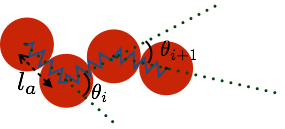
\includegraphics[width=\textwidth]{figs/figure2/filament_diagram.png}
    \caption{\label{fig:sketch}}
  \end{subfigure}
  ~
  \begin{subfigure}{0.4\textwidth}
    \centering
    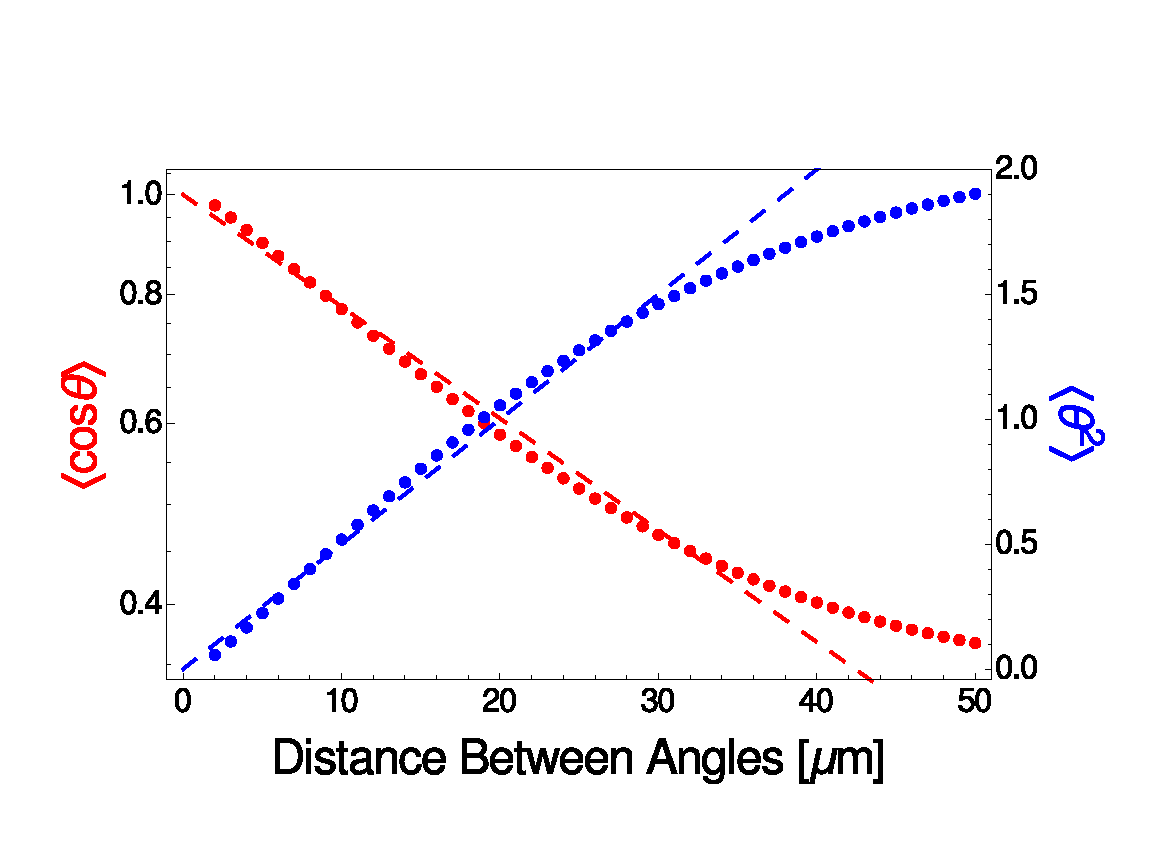
\includegraphics[width=\textwidth]{figs/figure2/ccf_th2_combo.eps}
    \caption{\label{fig:avgTh}}
  \end{subfigure}
  ~
  \begin{subfigure}{0.4\textwidth}
    \centering
    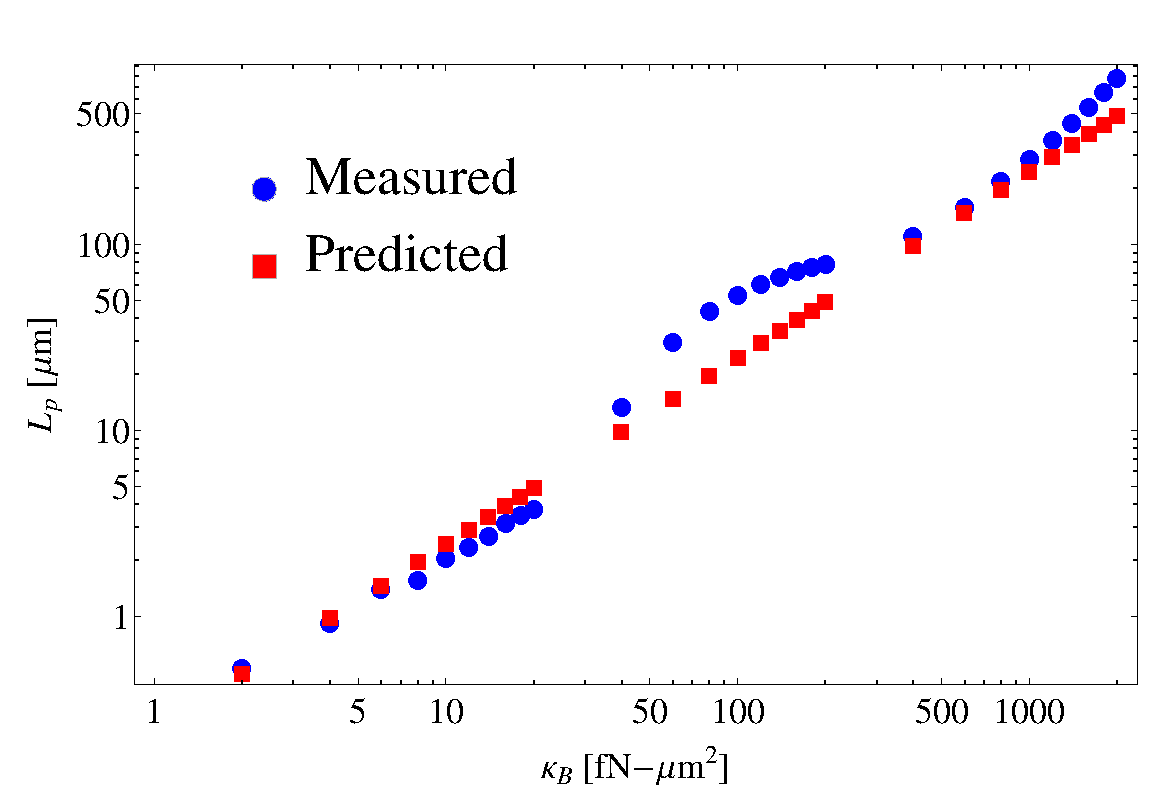
\includegraphics[width=\textwidth]{figs/figure2/kb_vs_lp_fit_all.eps}
    \caption{\label{fig:kb}}
  \end{subfigure}
  ~
  \begin{subfigure}{0.4\textwidth}
    \centering
    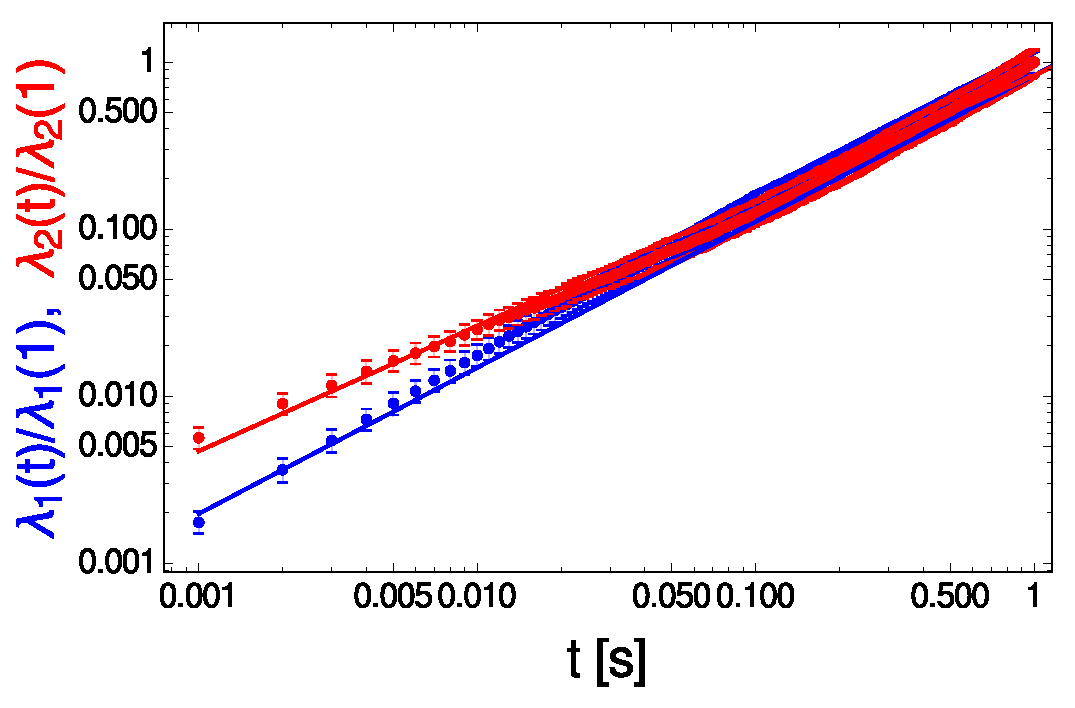
\includegraphics[width=\textwidth]{figs/figure2/lambda_v_t_no_leg_s1-100_sm.eps}
    \caption{\label{fig:fluc}}
  \end{subfigure}
  \caption{\label{fig:filament}
  Actin filament description. 
 \subref{fig:sketch} Sketch of the bead spring chain, illustrating the model.
  \subref{fig:avgTh} Decorrelation of tangent vectors (red dots) and fluctuations in angles between links (blue dots) 
  as a function of the arc length between them. Red dashed
  line is $e^{-s/2L_p}$ shows the expected behavior from the input bending modulus of $0.08 pN-\mu m^2$ and blue
  dashed line has slope $1/L_p$.
  \subref{fig:kb} Input bending modulus vs measured persistence length over three orders of magnitude. Persistence
  length was measured by fitting a line to $\ln{(\langle \cos{(\theta)}\rangle)}$ in each case.
  \subref{fig:fluc} Eigenvalues of covariance matrices for the positions of endpoints of filaments as a function of time. The blue
  dots shows the longitudinal fluctuations and the red dots shows the transvers fluctuations. Red dashed line is
  $t^{3/4}$ and blue dashed line is $t^{7/8}$ as predicted by \cite{everaers1999}. 
}
\end{figure} 
\subsection{Crosslinkers}
Crosslinker proteins dynamically connect actin filaments, thereby propogating force from one to
another. Thus model crosslinkers, must be able to attach and detach from actin filaments,
and be compliant in order to propagate force. They are therefore modeled as hookean springs, with stiffness
$k_{cl}$ and rest length $l_{cl}$. Like actin filaments, the Young's modulus of
most crosslinkers is significantly higher than would be reasonable to simulate; therefore we set $k_{cl} = 1-100pN/\mu m$ was
so that the bending mode of actin filaments was signicantly softer than the stretching mode of
crosslinkers. Their rest length $l_{cl}$ differs by the type of cross-linker and ranges from $~10 nm$ for fascin to $150 nm$
for filamin. 
\par
At each time step of the simulation an unattached crosslinker head is allowed to attach to nearby
filaments and an attached crosslinker head can detach. 
The probability of a head attaching to an actin filament is a Gaussian distributed random variable, such that
\begin{equation}
  P_{cl}^{on} = k_{cl}^{on}dt\exp(-r^2/R^2)
  \label{eqn:cl_on}
\end{equation} 
where $r$ is the shortest distance from the head to the actin filament and $R = \sqrt{2k_B T\over k_{cl}}$ 
where $k_B$ is Boltzmann's constant and $T$ is the temperature. 
For crosslinker detachment we assume that the behavior is that of a slip bond, such that a higher
tensile force along the crosslinker backbone will result in a higher probability of detachment. Thus, 
\begin{equation}
  P_{cl}^{off} = k_{cl}^{off} dt\exp{\left(  F x_{cl}/k_B T\right)}  
  \label{eqn:cl_off}
\end{equation}
where $F$ is the force along the crosslinker backbone, and $x_{cl}$ is a characteristic bond length \cite{stam2015}. 
\par
When a crosslinker is bound to a filaments at both ends, it will necessarily be stretched or compressed. 
If it were allowed to relax independently of the actin filaments to which it is bound. 
it would no longer lie on those filaments. Therefore, the tensile force stored on a stretched or compressed
crosslinker is propagated onto those actin filaments via the lever rule outlined in 
\cite{nedelec2002, gordon2012}. Thus, if the tensile force of a motor at point $r_j$ between filament beads $i$ and $i+1$ is
$F_{cl}$, then, 
\begin{eqnarray} 
  F_i &=& F_{cl}\left|\left( {r_j - r_i \over r_{i+1} - r_i }\right)\right|\\\nonumber
  F_{i+1} &=& F-F_i 
  \label{eqn:lever}
\end{eqnarray}
will be the forces on beads $i$ and $i+1$ respectively due to the crosslinker.
\subsection{Motors}
Within the cytoskeleton, tens of myosin II motors aggregate into bipolar ensembles called myosin minifilaments
\cite{stam2015}. While the mechanochemical process through which individual myosin motors walk along actin filaments is complex, 
motility assay experiments have shown that on average bound myosin II heads walk at an unloaded speed of $v_0\approx1\mu m/s$ along actin
filaments\cite{finer1994}. To a first approximation, minifilaments therefore should also 
have a mean speed of $1\mu m/s$ (although see \cite{stam2015} and \cite{walcott2012} for higher order measurements). 
Since myosin also functions to increase the local elasticity of networks wherever it is bound, the myosin is modeled
similarly to a crosslinker, in that it behaves like a hookean spring with two heads, a stiffness $k_{m}$ and a rest
length $l_m$. It should be noted, however, that the two heads of this spring do not correspond directly to individual
molecular myosin heads; rather each of them represents tens of myosin molecules, and their rate constants will reflect
that notion. 
It would be undesirable for a myosin minifilament to stretch, 
since experimentally they have a very high
Young's modulus and it is unlikely that their length would change noticably in the cytoskeleton. Thus we set $k_m\gg\kappa_B/l_a$
so that the bending of actin is still the softest mode. 
The rest length was set to the average length of minifilaments \cite{niederman1975}.
Attachment and detachment kinetics for motors are the same as for crosslinkers, subscripted with $m$
instead of $cl$ in \Cref{eqn:cl_on,eqn:cl_off}. One extra parameter is needed $k_m^{end}$ for the
detachment of myosin from the barbed end of a filament, as detachment from the end is significantly more probable than
from the rest of the filament.
Similarly, force propogation onto minifilaments is done using the lever rule described in \Cref{eqn:lever}.
\par
Unlike crosslinkers, motors precess towards the barbed end of actin filaments to which they are bound 
at speeds that vary depending on the tensile force along the crosslinker. 
The relationship between motor velocity and tensile force is modeled linearly, such that the motor head 
will speed up if the minifilament is
compressed (pre-powerstroke) and slow down if the minifilament is stretched (post powerstroke) going to
$0$ when the force on the minifilament is the stall force $F_s\approx 3.85pN$ \cite{nedelec2002, gordon2012}; i.e.,  
\begin{equation} 
  v(F_{||}) = v_0\left( 1-{F_{||}\over F_s}) \right)
    \label{eqn:myo_vel}
\end{equation} 
where $F_{||}$ is the force on the motor, projected along the tangent vector of the
actin filaments.
The minor differences between crosslinkers and motors allow us treat them equivalently, by 
setting $v_0 = 0$ for the crosslinkers.  
\subsection{Dynamics}
We use overdamped Langevin dynamics to solve for the motion of actin filaments, myosin minifilaments and crosslinkers.
The Langevin equations of motion for a spherical bead of
mass $m$, radius $R$ at position $r(t)$ at time $t$, being forced by an external force $F(t)$ is
\begin{equation}
  m\ddot{r}(t) = F(t) + B(t) - 4\pi R\nu \dot{r}(t)
  \label{eqn:lang}
\end{equation} 
where $B(t)$ is Brownian forcing term, to simulate a temperature, $\nu$ is the dynamic viscosity of the bead's
environment, and we have used the Einstein relation for the damping term.  
Since the fastest motion in this simulation is that of the myosin, and a $0.4\mu m$ myosin minifilament moving at
a speed of $1\mu m/s$ in a liquid at least as viscous as water ($\nu_D=10^6\mu m^2/s$ dynamic viscosity) has a very low Reynold's
number ($Re \approx 4*10^{-7}$) we assume the dynamics are overdamped and set $m=0$ in \Cref{eqn:lang}.
Furthermore, in the limit of small $\Delta t$, we may write $\dot{r(t)} \approx {r(t+\Delta t)-r(t)\over \Delta t}$. These two
approximations allow us to rewrite \Cref{eqn:lang} as 
\begin{equation}  
  r(t+\Delta t) = r(t) + F(t)\mu \Delta t + B(t) \mu \Delta t
  \label{eqn:overdamped}
\end{equation}
where $\mu = (4\pi R\nu)^{-1}$. For the brownian term, we use the form of Leimkuhler and Matthews \cite{leimkuhler2013} that has
been shown to minimize deviations from canonical averages in harmonic systems,
\begin{equation}
  B(t)=\sqrt{2k_BT\over\mu \Delta t}\left({W(t)+W(t-\Delta t)\over2}\right)
  \label{eqn:baoab_brownian}
\end{equation} 
where $W(t)$ is a Wiener process, in this case a random number drawn from the normal distribution $N(0,1)$. 
\subsection{Environment}
\par
Because the probability of motor attachment drops off exponentially as the distance squared from a filament, it is
highly inefficient to check for motor attachment for every filament in the simulation. Rather, a cutoff distance
$r_c>3R/2$ (where $R$ is defined above for \Cref{eqn:cl_on})
is determined such that if the distance between a motor and a filament is greater than $r_c$ the probability of
attachment is assumed to be $0$. A grid of lattice size $2r_c$ is drawn on the
$2D$ plane of the simulation, and the position of a filament is approximated as the points on the grid nearest to the
beads of the filament. Thus, to determine if a motor will bind to a filament at time $t$, it is sufficient to
only attempt attachment to filaments that are indexed at the four nearest grid points to a motor. 
\par
In general we use periodic boundary conditions so as to limit effects of a boundary and to mimic a system larger than
the one we simulate. Rigid boundaries as well as Lees-Edwards boundaries for shearing simulations have also been
implemented. The value for $\Delta t$ in \Cref{eqn:overdamped} generally depends on both the unloaded myosin speed
$v_0$ and the largest stiffness in the simulation $k_f$. For $k_f = 10pN/\mu m$ and $v_0=1\mu m/s$ a value of $\Delta t =
0.00001 s$ was low enough to iteratively solve \Cref{eqn:overdamped} without accumulating large error. 
The length and width of the simulations were chosen so as to be high enough to avoid boundary artifacts. 
A complete list of simulation parameters chose for each experiment can be seen in \Cref{tab:params}. 
\begin{table}
  \caption{Parameter Values}
  \centering
  \begin{tabular}{|C{1cm}|L{6cm}|C{2cm}|C{2cm}|C{2cm}|C{2cm}|}
    \hline\hline
    Symbol & Description (units) [ref] & $L_p$ & Shear & Motility Assay & Networks\\
    \hline
    &\bf{Actin Filaments}& & & &\\
    \hline
    $N_B$ & Number of beads & $21-201$ & $16$ & $16$ &$16$\\
    $l_a$ & Link Rest Length ($\mu m$)\cite{odijk1983}& $1$ & $1$ &$1$& $1$\\
    $k_a$ & Stretching Force Constant ($pN/\mu m$) & $0.01-10$ & $10$ & $1$ & $1$\\
    $\kappa_B$ & Bending Modulus ($pN\mu m^2$)\cite{ott1993} & $0.002-5 $ & $0.08$ & $0.08$ & $0.08$\\
    \hline
    &\bf{Myosin Minifilaments}& & \\
    \hline
    $l_m$ & Rest Length ($\mu m$)\cite{niederman1975} & n/a & n/a & 0.5 & 0.5\\
    $k_m$ & Stiffness ($pN/\mu m$)& n/a & n/a & $1$ & $1$\\
    $k^{on}_m$ & Attachment rate at distance $r=0$ ($s^{-1}$)& n/a & n/a &$2-4000$ &$3600$\\
    $k^{off}_m$ & Unloaded head detachment rate ($s^{-1}$)& n/a & n/a & $200$ &$200$\\
    $k^{end}_m$ & Unloaded head detachment rate at the barbed end of the filament ($s^{-1}$)& n/a & n/a &$2000$ &$2000$\\
    $x_m$ & characteristic bond length ($\mu m$) \cite{stam2015}& n/a & n/a & $0.0004$& $0.0004$\\
    $v_0$ & Unloaded speed ($\mu m/s$) \cite{kron1986}&  n/a & n/a & $1$ & $1$\\
    $F_s$ & Stall force of myosin ($pN$)\cite{veigel2003}& n/a & n/a & $3.85$ & $3.85$\\
    \hline
    &\bf{Crosslinkers} & & \\
    \hline
    $l_{cl}$& Rest Length (Filamin) ($\mu m$)\cite{ferrer2008} & n/a &$0.150$ &n/a&$0.150$ \\
    $k_{cl}$ & Stiffness ($pN/\mu m$)& n/a & $1,10$ & n/a& $1$\\
    $k^{on}_{cl}$ & Attachment rate at distance $r=0$ ($s^{-1}$)& n/a & $10^6,10^5$ &n/a &$3600$\\
    $k^{off}_{cl}$ & Unloaded head detachment rate ($s^{-1}$)& n/a & 0 & n/a&$0.2$\\
    $x_{cl}$& characteristic bond length ($\mu m$) & n/a & $0.0004$ & $0.0004$ & $0.0004$ \\
    \hline
    &\bf{Environment} & & \\
    \hline
    $dt$ & Dynamics timestep (s) & $10^{-4}$ & $10^{-6},10^{-5}$ &$2.5\times10^{-4}$ &$2.5\times10^{-4}$ \\
    $T_F$& total simulated time (s) & $100$ & $0.5$ & $100$ & $500$ \\
    $X$, $Y$ & Length and width of assay ($\mu m$)& n/a & $75$ & $50$ & $75$\\
    $r_c$ & Mesh (actomyosin binding site) size ($\mu m$) & $n/a$ & $0.2 $ & $0.2 $& $0.2 $ \\ 
    $T$ & $k_B$ * Temperature ($pN\mu m$)& $0.004$ & $0.004$& $0.004$& $0.004$\\
    $\nu$ & Dynamic viscosity ($mg/(\mu m s)$) & $0.001$& $0.001$& $0.001$& $0.001$\\
    $\gamma$ & Strain (\%) \cite{stricker2010}& n/a& $0.001$&n/a&n/a\\
    $t_{relax}$ & Amount of time between sequential strains (s)& n/a& $0.001$ &n/a&n/a\\
    \hline
  \end{tabular}
  \label{tab:params}
\end{table}
\section{Comparison to Expected Results}
\subsection{Actin Filaments Exhibit Predicted Spatial and Temporal Fluctuations}
For a two dimensional filament composed of links $d_1..d_N$ with a constant link length $l_a$, constant total contour
length $L$, and where a small bend of link
$d_i$ with respect to link $d_{i-1}$ will result in a local change in free energy of ${\kappa_B\over2l_a\theta_i^2}$, it
is possible to show explicitly that \cite{frontali1979}
\begin{equation}
  \langle\theta^2(l)\rangle = {l_a\over L_p}
  \label{eqn:thsq}
\end{equation}
\begin{equation} 
  \langle\cos(\theta(l))\rangle = \exp{(-l_a/2L_p)}
  \label{eqn:costh}
\end{equation} 
where $\theta(l) = \theta_j - \theta_i$ where $1<i<j\le N$, $l = l_a(j-i)$ and $L_p$ is the persistence length. 
To test our WLC model against these equations, we let $100$ filaments of $L=200\mu m$ and $\kappa_B=0.08 pN\mu m^2$ fluctuate at
$T=300K$ for $T_f = 100s$ and measured the resulting filament configuration every $1s$, as that was more than enough
time for configurations to decorrelate. The first $10$ seconds of each simulation was disregarded as filaments had not
yet equilibrated, and the first and last $25\mu m$ of each filament were disregarded because of possible boundary
effects. 
For each of the $90000$ filament configurations, and for each $l\in{0,1,2,..,150}\mu m$,
$\theta^2(l)$ and $\cos(\theta(l))$ were calculated, and their respective averages are plotted in 
\Cref{fig:avgTh}, along with the expected behavior given the input $\kappa_B$.  \Cref{fig:kb} shows that the
measured persistence length, obtained by performing a least squares fit to plots of
 $\log{(\langle cos(\theta(l))\rangle )} $
 for various values of $\kappa_B$ yields the expected result over at least $3$
orders of magnitude. Further measurements of the persistence length as well as verifications of its independence on
other filament parameters is available in the supplement \Cref{lpCalc}.

\par
Another benchmark for semiflexible filaments were the fluctuations in time. 
Fluctuations transverse to the filament orientation have been 
shown to increase as a function of time as $\langle dr_{\perp}^2\rangle\propto t^{3/4}$ while longitudinal fluctuations have been shown to follow the power law
$\langle dr_{||}^2\rangle\propto t^{7/8}$ \cite{everaers1999}. To tests these predictions, we followed the procedure outlined in
\cite{everaers1999} and generated $N = 100$ initial filament configurations of a $20\mu m$ filament. For each configuration
we ran $M = 100$ simulations of the filament fluctuating for $1s$. At each timestep each of the two ends of the
filament thus had $M$ possible position $r_e(t)$. For each of these clouds of points, we calculated
the moments, as the eigenvalues of the covariance matrix $cov(r_e(t)\cdot \hat{i},r_e(t)\cdot \hat{j})$ where
$i,j\in\{x,y\}$.
The larger eigenvalue $\lambda_1(t)$ corresponds to the longitudinal fluctuations
(i.e., $\lambda_1(t)\propto t^{7/8}$) while the smaller eigenvalue corresponded to the perpendicular fluctuations
($\lambda_2(t)\propto t^{3/4}$). We show these results in \Cref{fig:fluc}. Each data point is the
average over the $2N$ eigenvalues for $\lambda_1(t)$ and $\lambda_2(t)$ while the error bars are the standard deviations for the
distribution of these values. As seen, they are in good agreement with the predicted behavior. 
\subsection{Passive F-actin Crosslinked Networks Exhibit Predicted Viscoelasticity}
\par
The material properties of cross-linked F-actin networks are generally characterized using rheology. In a common
experiment, actin and crosslinker proteins are mixed and form a crosslinked mesh. The mesh is placed in a rheometer and then 
sheared by a prestress $\sigma_0$. The prestressed network then undergoes a sinusoidal differential stress of magnitude
$d\sigma<<\sigma_0$. By measuring the resulting strain, one can calculate the
differential elastic modulus $G(\sigma_0) = {d\sigma\over d\gamma}$. 
In experiments using a stiff crosslinker, such as scruin, the dependance of the differential modulus on high prestress 
is $G\propto\sigma_0^{3/2}$, indicating that this shear stiffening results from the nonlinear response of
stretching actin \cite{gardel2004,lin2010}. Experiments using more compliant crosslinkers, such as filamin, have found a softer
stiffening response, $G\propto\sigma_0$, indicating that a significant amount of stress is going into the crosslinkers,
and not the actin\cite{kasza2009}.
\par
We used these experimental results to benchmark our simulation. 
$24$ passive networks were simulated by randomly orienting $N = 500$ $15\mu m$ filaments on a $75\mu m \times 75\mu m$ square. A
$0.150\mu m$ cross link (corresponding to the length of filamin) was initially placed at each intersection of links on
different filaments and attached to both filaments. The detachment rates of the crosslinkers was set to zero. 
An affine strain of $\gamma=0.001$ was applied such that the horizontal position of every actin bead ($x_a$) was shifted 
\begin{equation}
  x_a \rightarrow x_a + \gamma \left( {y_a\over Y} \right)
  \label{eqn:sllod}
\end{equation} 
following the overdamped SLLOD equations of motion \cite{evans1984}. The periodic boundary was simulatenously shifted
following the the Lees-Edwards convention \cite{allen}. The mesh was then allowed to relax for $t_{relax} =
1 ms$ before the next strain of $\gamma$. This was performed for $T_f=0.5s$ so that the total strain was
$\gamma T_f/t_{relax}=0.5$. Increasing $t_{relax}$ did not significantly change the simulation
results as seen in \Cref{fig:tRelax10}.  
\par
The shear modulus at each strain was measured by calculating $w$, the strain energy density at each timestep
\begin{equation}
  w(t) = {1\over X Y}\left(\sum_f{ U_f}+\sum_{cl}{U_{cl}}\right)
  \label{eqn:sed}
\end{equation}
where $U_f$ is defined in \Cref{eqn:Ufil} and $U_{cl}$ is the potential energy of each cross link, averaging
over windows of size $t_{relax}$ to obtain $w(\gamma)$ and taking the second derivative $G = {d^2w\over d\gamma^2}$ using a finite
difference approximation. \Cref{fig:strain_stiffening} shows the results of these calculations for two different
crosslinker stiffnesses. For the softer crosslinker, with $k=10pN/\mu m$, it was observed that $G\propto\gamma$ while
for a stiffer crosslinker stiffness $k=100pN/\mu m$, $G\propto\gamma^{3/2}$ matching the strain
stiffening differences observed in the experiments of \cite{gardel2004} and \cite{kasza2009}. However, our
simulation can also provide further insight into this experiment, because we can measure the relative contributions to
the strain energy from filament stretching, filament bending, and crosslinker stretching. These results are plotted in
\Cref{fig:energy_contribs} and show that in the case of the stiffer crosslinker, more of the strain energy is stored in the
crosslinks, and less is stored in the filaments, than at lower crosslinker stiffness. 

\begin{figure}[H]
  \begin{subfigure}{0.3\textwidth}
    \centering
    \includegraphics[width=\textwidth]{figs/elasticity/strain_mid.eps}
    \caption{\label{fig:lees-edwards}}
  \end{subfigure}
  ~
  \begin{subfigure}{0.4\textwidth}
    \centering
    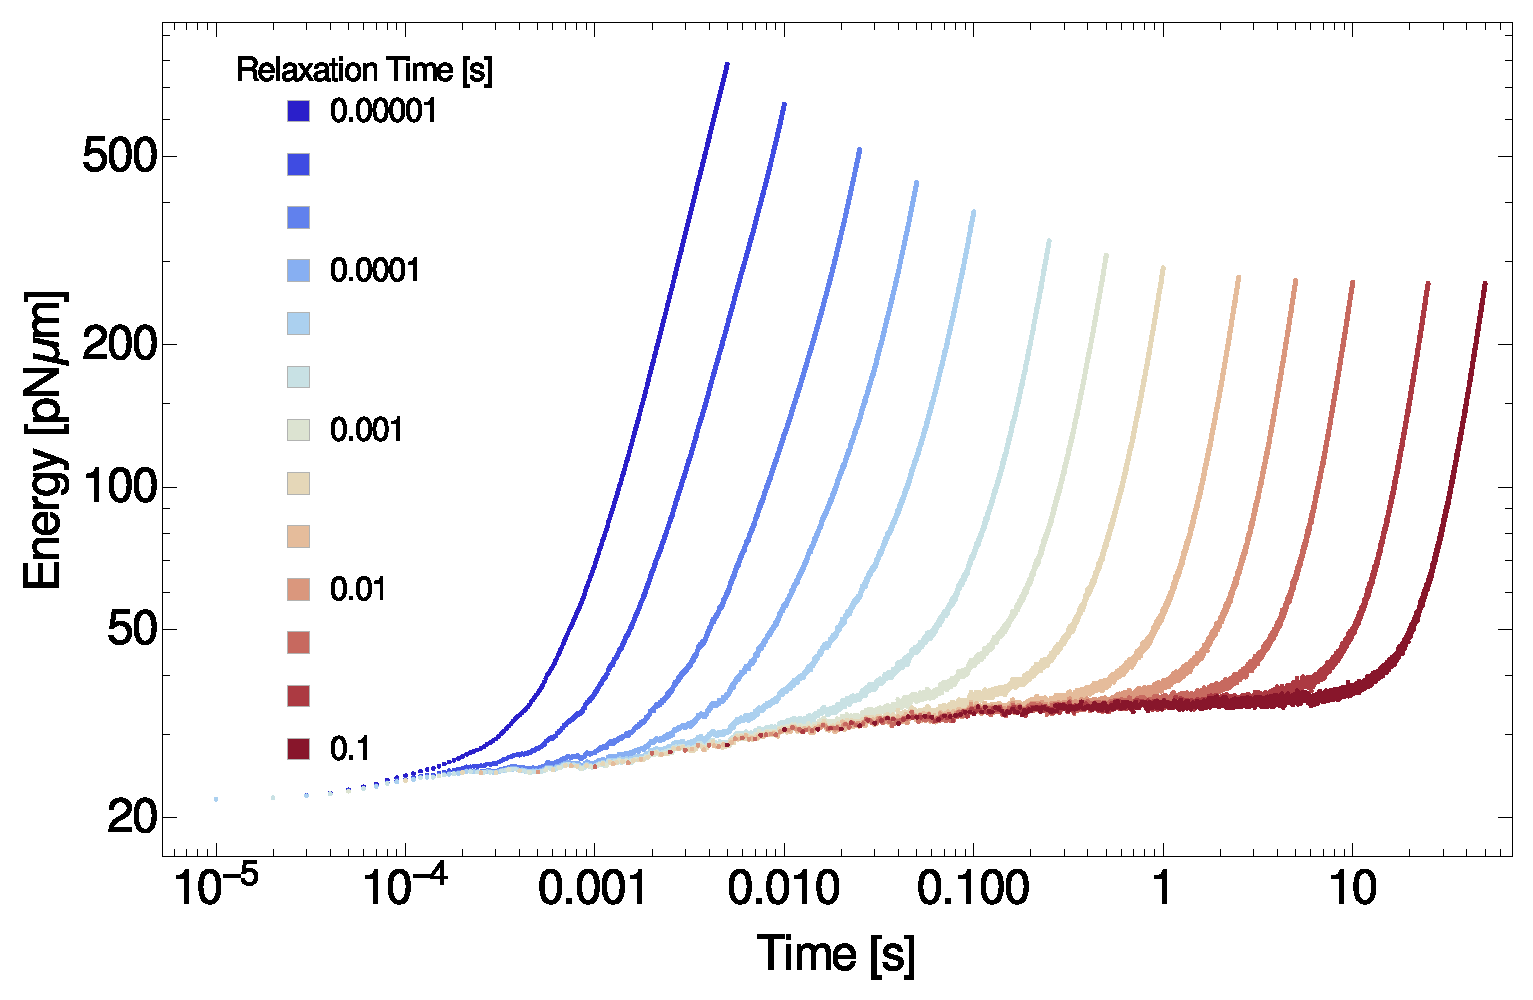
\includegraphics[width=\textwidth]{figs/elasticity/eng_vs_t_k10.eps}
    \caption{\label{fig:tRelax10}}
  \end{subfigure}
  ~
  \begin{subfigure}{0.5\textwidth}
    \centering
    \includegraphics[width=\textwidth]{figs/elasticity/strain_stiffening_soft_and_hard.eps}
    \caption{\label{fig:strain_stiffening}}
  \end{subfigure}
  ~
  \begin{subfigure}{0.5\textwidth}
    \centering
    \includegraphics[width=\textwidth]{figs/elasticity/eng_pcts_vs_time.eps}
    \caption{\label{fig:energy_contribs}}
  \end{subfigure}
  \caption{%
    \label{fig:stress}%
    \subref{fig:lees-edwards} One of the strained networks initiated at time $t= 0.5s$. Color indicates stretching energy
    on each link, with white being the lowest and red being the highest. \subref{fig:tRelax10} The strain energy as a
    function of time for the same network using different values of $t_{relax}$. The curves are indistinguishable for
    $t_{relax} \ge 1ms$. \subref{fig:strain_stiffening} The shear modulus as a function of time for stiffly (red) and softly
    (blue) crosslinked networks. The red dashed line shows $G\propto\gamma^{3/2}$ while the blue dashed line shows
    $G\propto\gamma$. \subref{fig:energy_contribs} Relative energy contributions for the stiffly (red) and softly (blue)
    crosslinked networks. The stretching energy of the filaments (circles) dominate in both cases, and is larger
    in the stiff case. The bending energy of the filaments (triangles) is nearly identical in both cases. The
    crosslinker stretching energy (squares) is higher in the soft crosslinker case.
  }
\end{figure}  
\subsection{Simulation Reproduces Experimental Results for Myosin Motility Assays}
While the force dependent detachment and speed of an individual myosin motor is well approximated by
the input behavior, specified in \Cref{eqn:cl_off,eqn:myo_vel}, the ensemble behavior of many
myosins is not input, and could provide a benchmark that the simulation is accurately representing active actomyosin
assays \cite{walcott2012}. One experiment involving an ensemble of motors is the motility assay, in which a layer of myosin is
adhered to a plate, and actin filaments are placed on top of the myosin. Because the myosin cannot diffuse, they instead
slide the actin filament across the assay.
Although this experiment typically involves single myosin heads, and not myosin minifilaments, we believe that
functionally the situations would be equivalent, with the substitution that each model motor head approximates the
activity of dozens of single molecule myosin heads. 
Various groups \cite{harris1993, umemoto1990} found a
nonlinear dependance of the speed of an actin filament across the assay on the concentration of myosin, the length of
the actin filament, and the concentration of ATP in the sample. By allowing filaments to interact with more motors, one
can increase the filament monotonically to a critical speed. 
\par
To explore this experiment, we randomly distributed motors on a periodic lattice and
constrained one head of each motor to remain in place. Filaments were then placed in the $50\mu m\times50\mu m$ simulation cell and 
allowed to interact with the unconstrained motor heads. The number of motor-filament interactions were explored in three
ways: by varying the motor concentration, the filament length, and the ratio $r_D = k_m^{on}/k_m^{off}$. 
The results are shown in \Cref{fig:motility}. 
\par
In general, the finding was qualitatively similar to the experimental findings. 
For low motor density, filament length and $r_D$, transverse filament fluctuations dominate over longitudinal ones as
it is not being propelled by motors faster than diffusion. However, as these variables are increase, longitudinal
fluctuations become dominant. Interestingly, the speed of the filament seems to plateau for filaments that are $>10\mu
m$, similar to experiments, perhaps for the same reason that as the filament gets longer there are less motors to
interact with each part of the filament. Similarly for $r_D\ge1$ the velocity is approximately constant, indicating that
velocity reaches its maximum when $P(attached) > P(detached)$.
\begin{figure}[H] 
  \begin{subfigure}{0.2\textwidth}
    \centering
    \caption{\label{fig:xt}$r_D = 0.01$}
    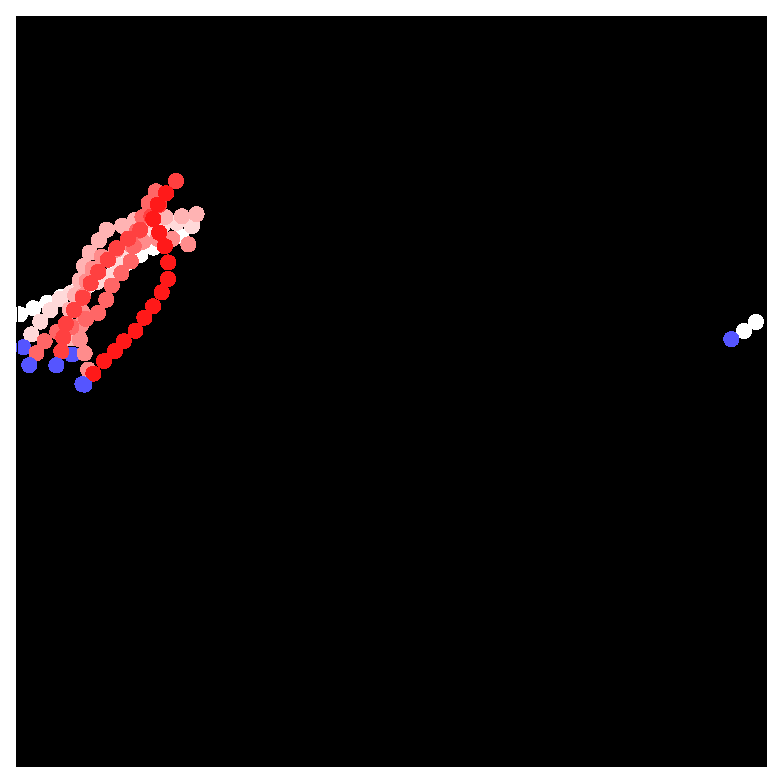
\includegraphics[width=\textwidth]{figs/motility/kon2_fil2.eps}
  \end{subfigure}
  ~
  \begin{subfigure}{0.2\textwidth}
    \centering
    \caption{$r_D = 0.1$}
    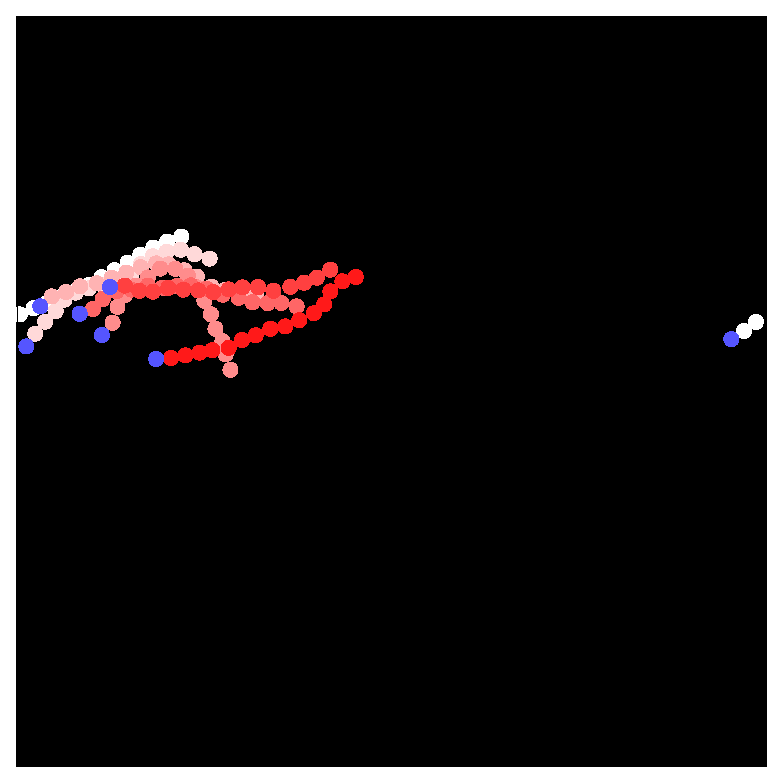
\includegraphics[width=\textwidth]{figs/motility/kon20_fil2.eps}
  \end{subfigure}
  ~
  \begin{subfigure}{0.2\textwidth}
    \centering
    \caption{$r_D = 1$}
    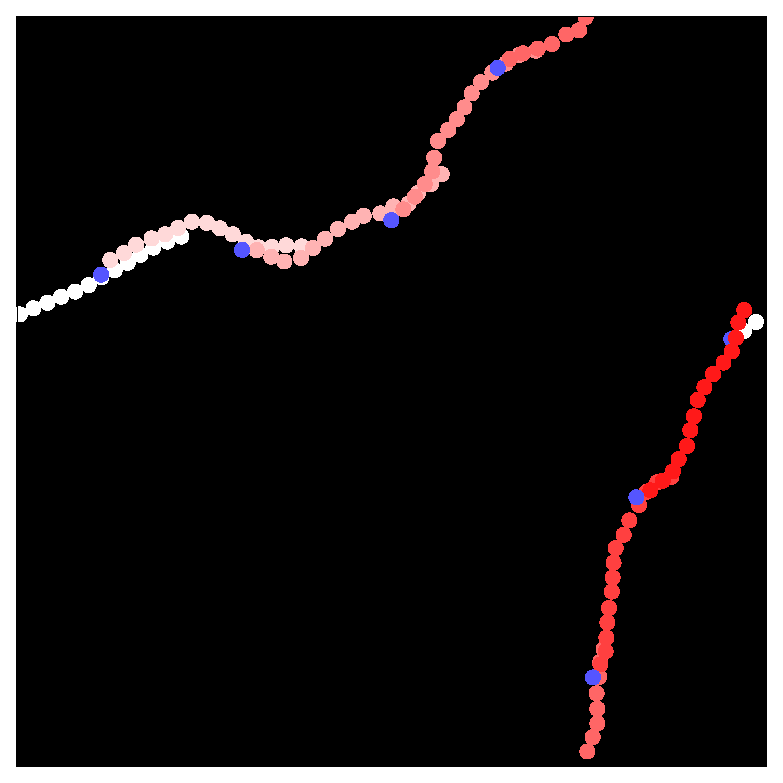
\includegraphics[width=\textwidth]{figs/motility/kon200_fil2.eps}
  \end{subfigure}
  ~
  \begin{subfigure}{0.2\textwidth}
    \centering
    \caption{\label{fig:xthi}$r_D = 10$}
    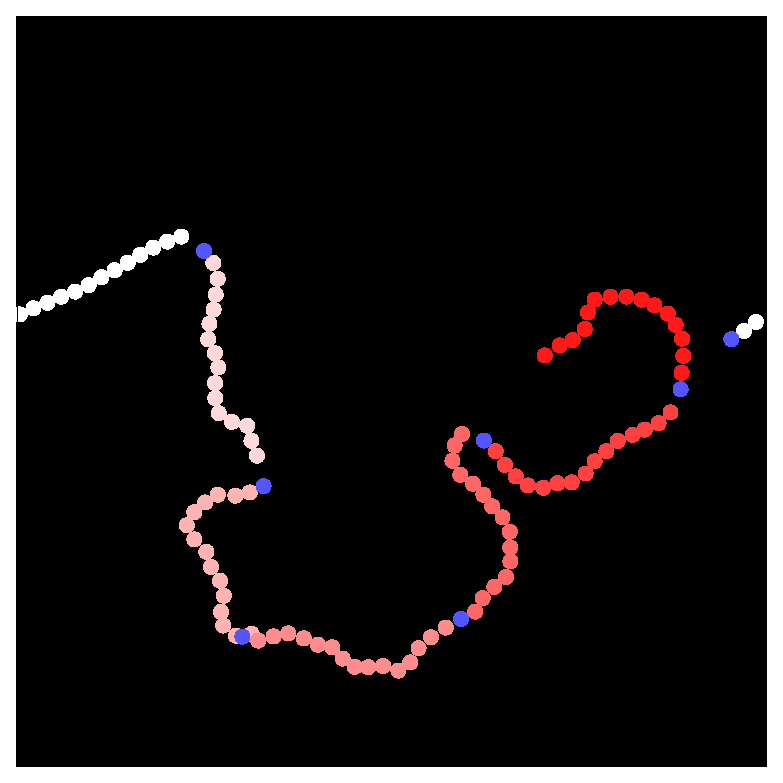
\includegraphics[width=\textwidth]{figs/motility/kon2000_fil2.eps}
  \end{subfigure}
  ~
  \begin{subfigure}{0.33\textwidth}
    \centering
    \includegraphics[width=\textwidth]{figs/motility/v_vs_density_no_leg.eps}
    \caption{\label{fig:v_vs_dens}}
  \end{subfigure}
  ~
  \begin{subfigure}{0.33\textwidth}
    \centering
    \includegraphics[width=\textwidth]{figs/motility/v_vs_L_no_leg.eps}
    \caption{\label{fig:v_vs_len}}
  \end{subfigure}
  ~
  \begin{subfigure}{0.3\textwidth}
    \centering
    \includegraphics[width=\textwidth]{figs/motility/v_vs_k_no_leg.eps}
    \caption{\label{fig:v_vs_k}}
  \end{subfigure}
  \caption{%
  \label{fig:motility}%
  Active Network Benchmarks. \subref{fig:xt}-\subref{fig:xthi} Position of a filament for $\rho_m = 10\mu m^{-2}$ and $L = 16\mu m$ for
  different values of the duty ratio. White filament is $t=0$ and dark red is $t=90s$. Blue dot marks the barbed end of filaments.  
  \subref{fig:v_vs_dens} Longitudinal filament speed (black squares) while transverse speed (orange circles) decreases with motor density 
  but does not asymptote due to no limit on binding sites. \subref{fig:v_vs_len} Longitudinal speed increases and
  plauteaus as seen in experiment. \subref{fig:v_vs_k} Duty ratio can be controlled directly in simulation to change the
  probability that a motor is bound to a filament, and tune the effective motor density. 
    }
\end{figure}
 
\section{Model Exhibits Emergent Contractility and Polarity Sorting}
The most striking biological function of actomyosin networks is their contractility, which results in muscle cell
contraction, and is instrumental in motility and division in non-muscle cells. 
That these complex macroscopic mechanisms arise stochastically from simple microscopic interactions suggests the ability
to engineer materials with controllable network topologies. 
Recently, in-vitro experiments of
reconstituted actomyosin networks have demonstrated this controllable architecture by varying motor density and
crosslinker density and showing how they effect contractility\cite{murrell2012, murrell2014}. Using our model,
we will show that we can manipulate these variables to further explore the dependance of contractility on these 
and other microscopic parameters. 
Additionally, we show that we can tune a different macroscopic organizational technique, called polarity sorting, 
in which motors align filaments by their polarity. 
\par
To reproduce contractile networks, $500$ $15\mu m$ filaments were placed on a $75\mu m\times 75\mu m$ simulation cell, and
crosslinked at their intersections. Motor density was varied between $0.1\mu
m^{-2}$ and $10\mu m^{-2}$. The crosslinkers were kept sticky with a low duty ratio, while the motors were highly active
with a high duty ratio. This ensured that connectivity of the network was almost exclusively controlled by crosslinkers
while force generation was controlled by motors. 
\par
The results of these networks can be seen in \Cref{fig:contract}. The effective contractility was measured by
interpolating a velocity field from the displacement vectors of filament beads, and measuring the divergence of the
velocity fields as is done in ref \cite{murrell2014}. A negative divergence indicates a contractile network. As evident
in \Cref{fig:div_vs_t}, higher motor density leads to larger contractility. \Cref{fig:div_vs_strain} shows
that actin buckling, here measured as the change in the end to end distance $s$ of an actin filament
\begin{equation}
  s = \left(1 - {|r_{15}-r_0|\over\sum_{i=1}^{15}{|r_i-r_{i-1}|}}\right) 
  \label{eqn:fil_strain}
\end{equation}
correlates with contractility, suggesting that the primary mechanism driving
contractility in these flexible networks is buckling, as seen in experiment \cite{murrell2012}. 
\begin{figure}[H] 
  \begin{subfigure}{0.25\textwidth}
    \centering
    \caption{\label{fig:rholo}$\rho_m=0.1$}
    \includegraphics[width=\textwidth]{figs/divergence/dens0-1.eps}
  \end{subfigure}
  ~
  \begin{subfigure}{0.25\textwidth}
    \centering
    \caption{$\rho_m=1$}
    \includegraphics[width=\textwidth]{figs/divergence/dens1.eps}
  \end{subfigure}
  ~
  \begin{subfigure}{0.25\textwidth}
    \centering
    \caption{\label{fig:rhohi}$\rho_m = 10$}
    \includegraphics[width=\textwidth]{figs/divergence/dens10.eps}
  \end{subfigure}
  ~
  \begin{subfigure}{0.32\textwidth}
    \centering
    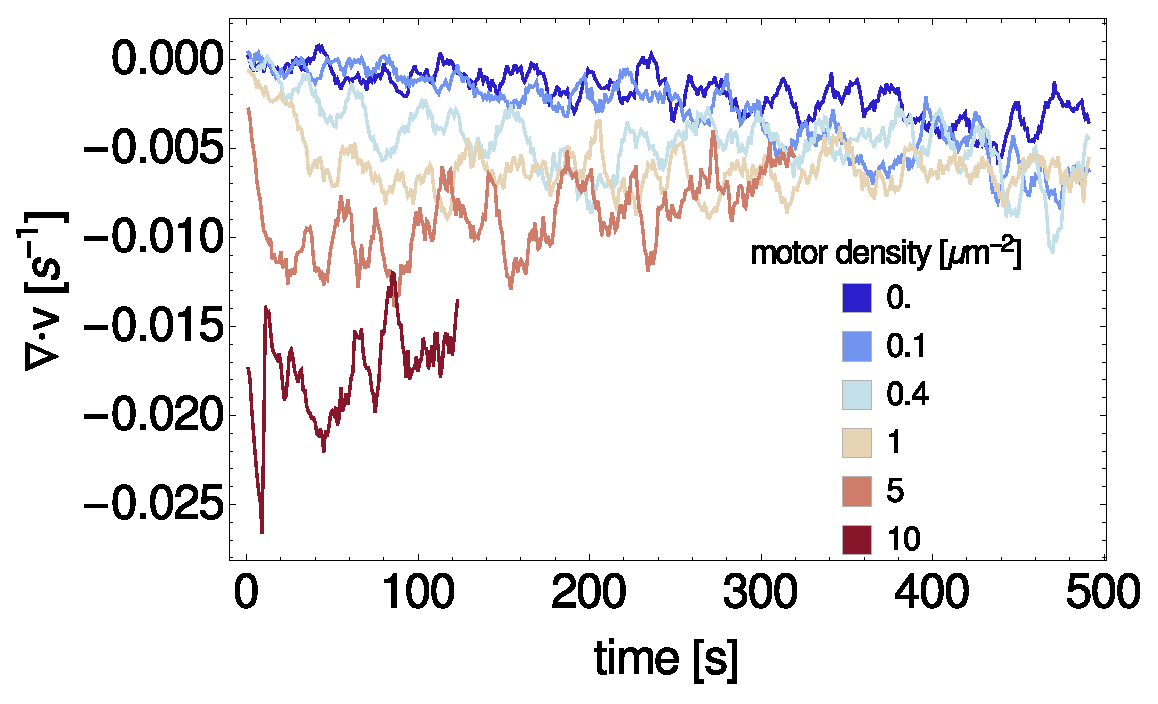
\includegraphics[width=\textwidth]{figs/divergence/divergence_vs_time_wleg.eps}
    \caption{\label{fig:div_vs_t}}
  \end{subfigure}
  ~
  \begin{subfigure}{0.32\textwidth}
    \centering
    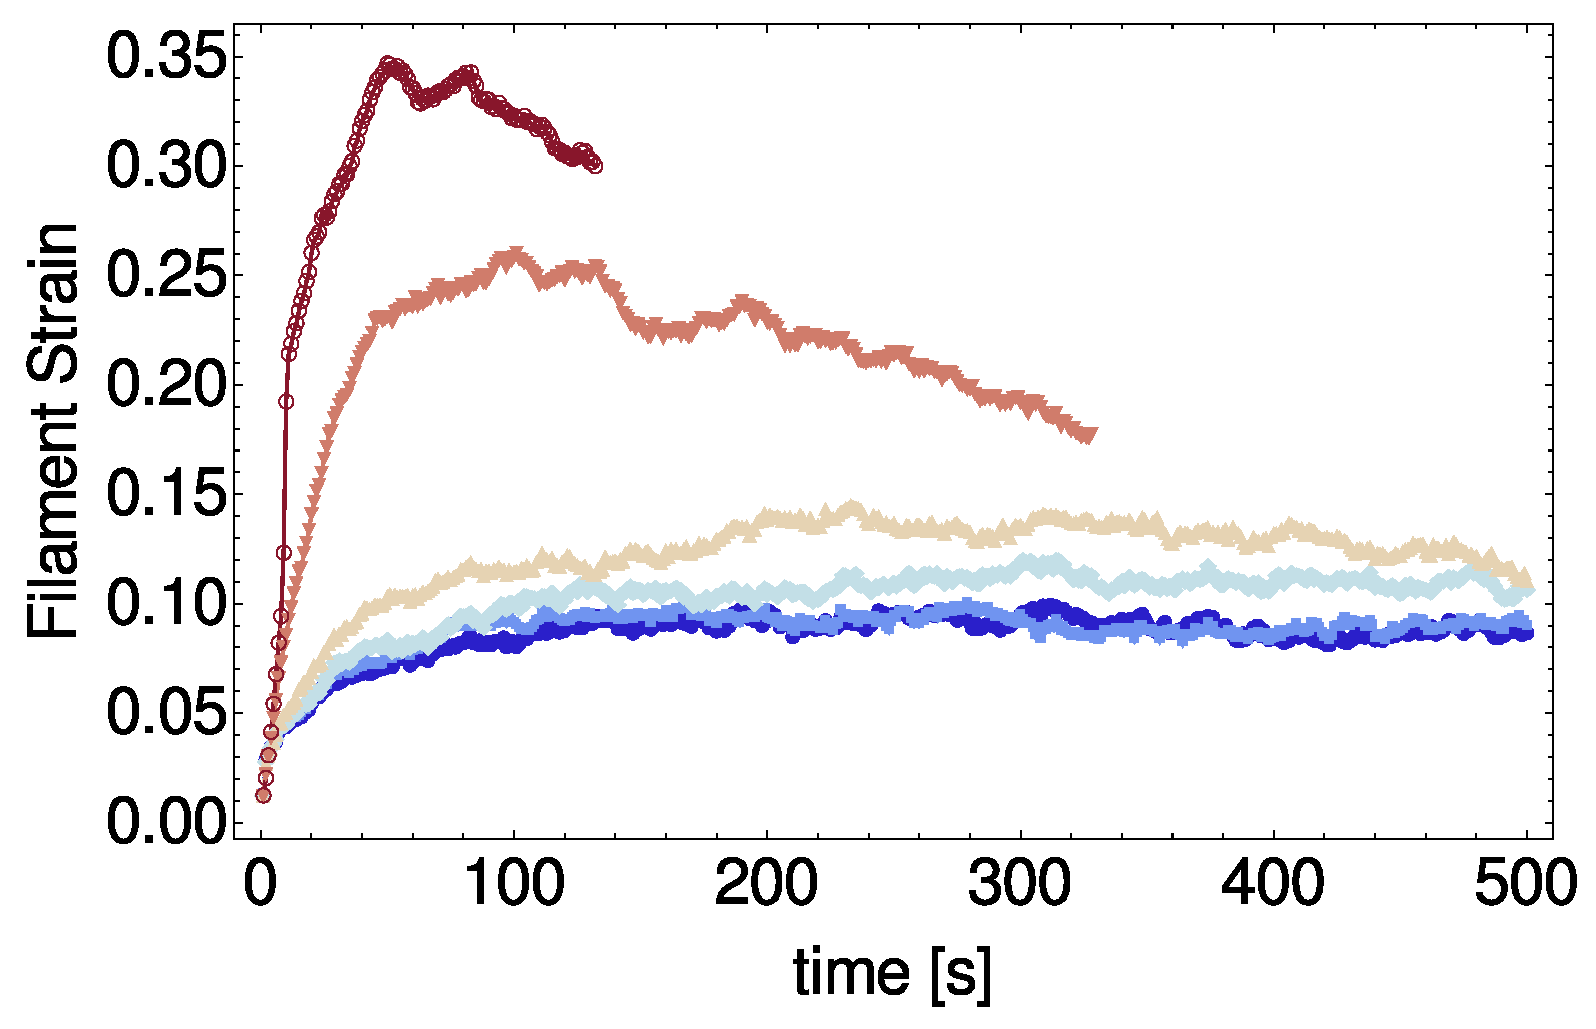
\includegraphics[width=\textwidth]{figs/divergence/strain_vs_t_select.eps}
    \caption{\label{fig:strain_vs_t}}
  \end{subfigure}
  ~
  \begin{subfigure}{0.32\textwidth}
    \centering
    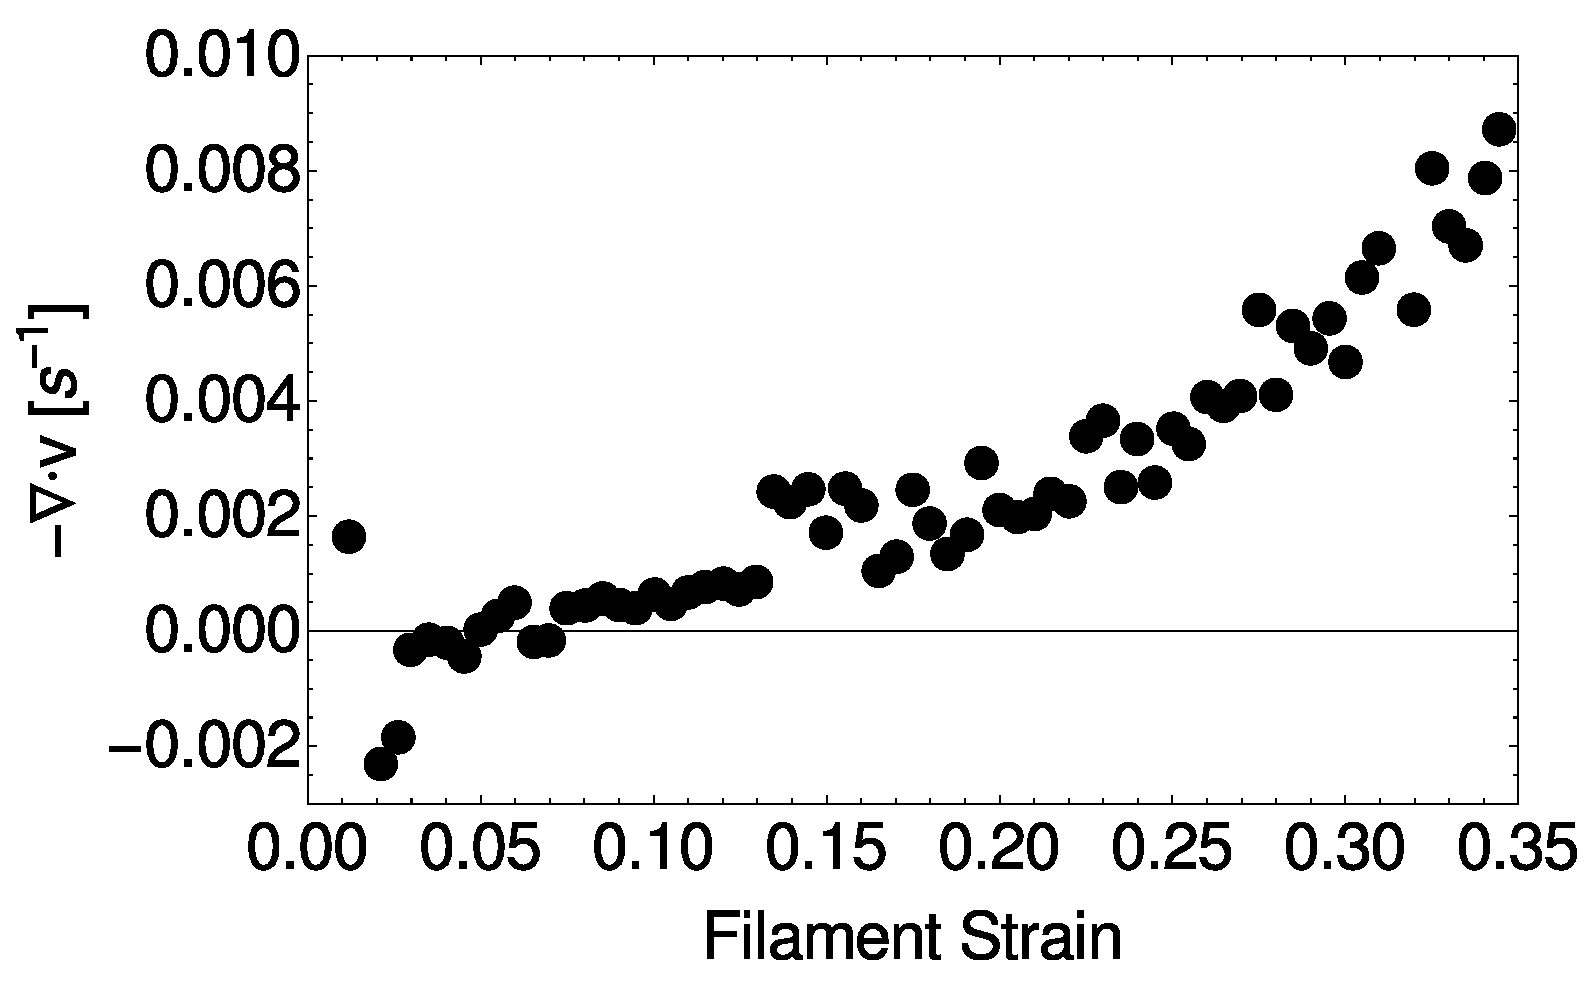
\includegraphics[width=\textwidth]{figs/divergence/div_vs_strain_avg.eps}
    \caption{\label{fig:div_vs_strain}}
  \end{subfigure}
  \caption{%
  \label{fig:contract}%
  Active Network Benchmarks. \subref{fig:rholo}-\subref{fig:rhohi} 
  Networks at their largest contractility. Filaments in red, motors in white. Only $1000$ motors are shown in each case.
  Blue dots marks the barbed end of filaments. \subref{fig:div_vs_t} Average divergence as a function of time for
  networks of varying motor density. Networks with a higher density of motors are more contractile.  \subref{fig:strain_vs_t}
  Average filament strain (defined in \Cref{eqn:fil_strain}) as a function of time for the same networks as in
  \subref{fig:strain_vs_t}. \subref{fig:div_vs_strain} Correlation between filament strain and network strain measured 
 negative of divergence for all times and all motor densities, averaged over bins of size $0.005$} 
\end{figure}
Without crosslinkers, simulated networks did not contract. However, there was a general
restructuring of the filaments in the form of polarity sorting. Motors would aggregate on the barbed ends of filaments
and thereby bring the barbed ends together, to form aster-like objects. The magnitude of polarity sorting was measured
by calculating the average distance of a motor from the barbed end of filaments. As seen from 
\Cref{fig:dist_vs_mdens}, increasing motor density had the effect of increasing polarity sorting, suggesting that this
form of restructuring is highly tunable. 
\begin{figure}[H] 
  \begin{subfigure}{0.3\textwidth}
    \centering
    \caption{\label{fig:rholops}$\rho_m=0.1$}
    \includegraphics[width=\textwidth]{figs/polarity_sorting/dens0-1.eps}
  \end{subfigure}
  ~
  \begin{subfigure}{0.3\textwidth}
    \centering
    \caption{$\rho_m=1$}
    \includegraphics[width=\textwidth]{figs/polarity_sorting/dens1.eps}
  \end{subfigure}
  ~
  \begin{subfigure}{0.3\textwidth}
    \centering
    \caption{\label{fig:rhohips}$\rho_m = 10$}
    \includegraphics[width=\textwidth]{figs/polarity_sorting/dens10.eps}
  \end{subfigure}
  ~
  \begin{subfigure}{0.43\textwidth}
    \centering
    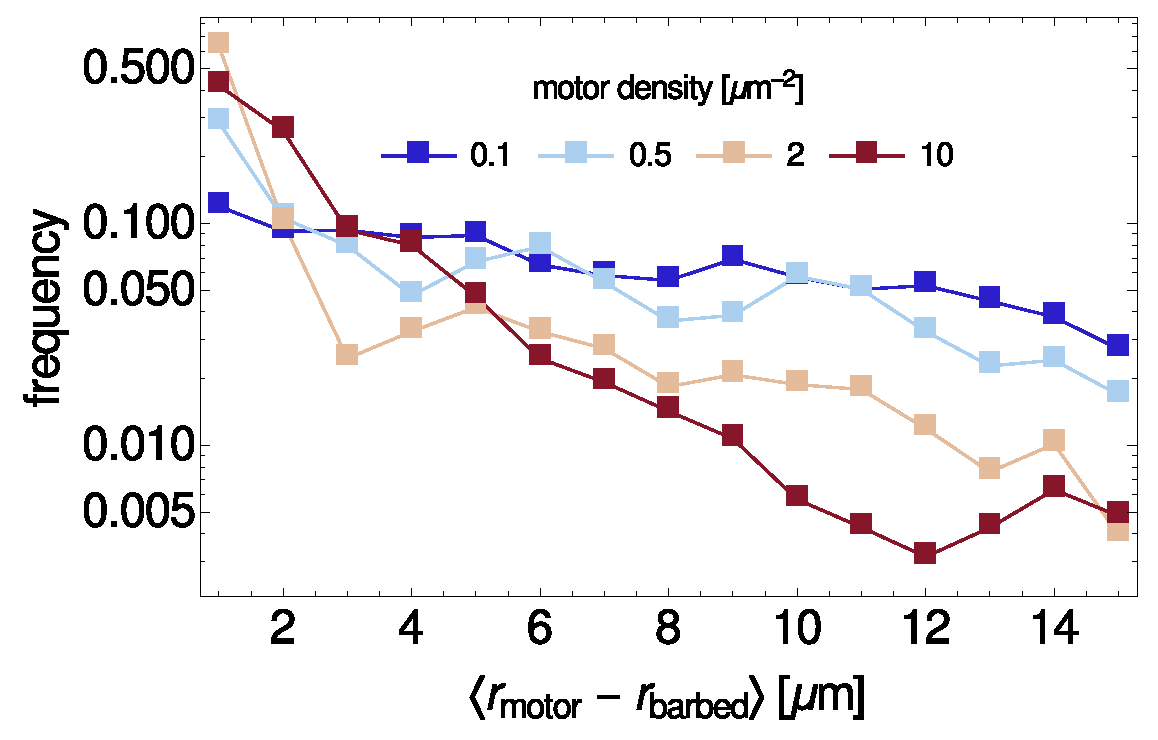
\includegraphics[width=\textwidth]{figs/polarity_sorting/dist_vs_freq.eps}
    \caption{\label{fig:dist_hist}}
  \end{subfigure}
  ~
  \begin{subfigure}{0.4\textwidth}
    \centering
    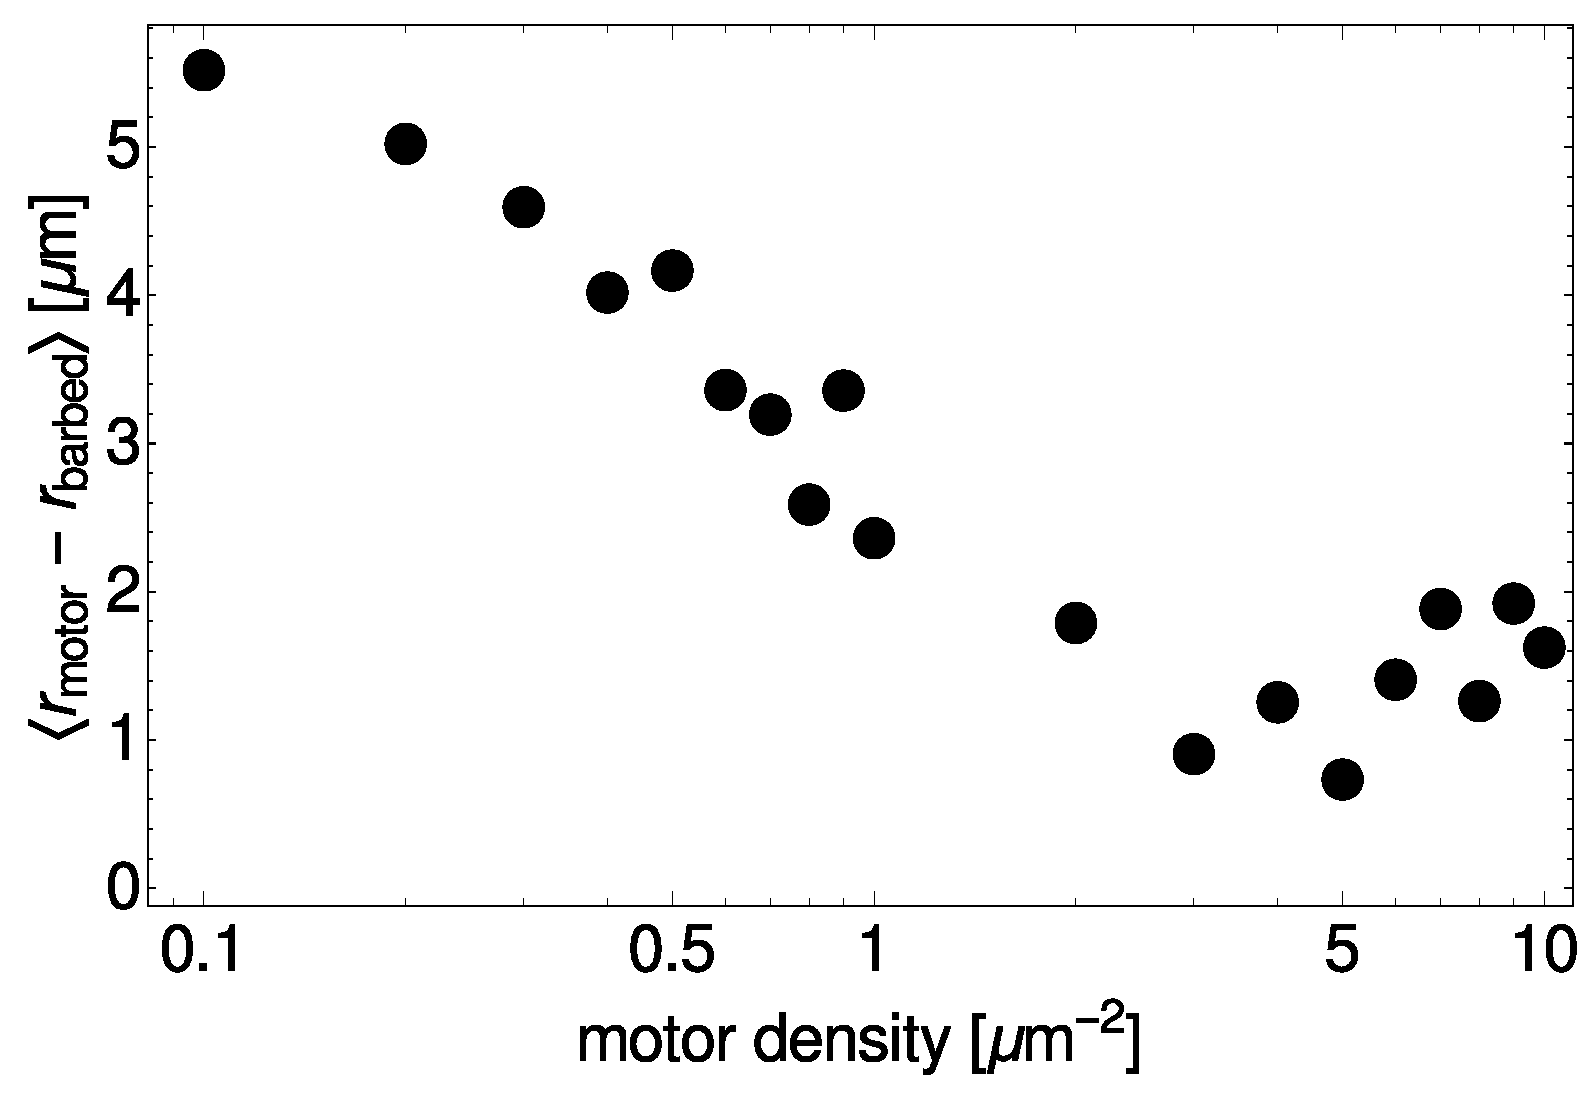
\includegraphics[width=\textwidth]{figs/polarity_sorting/dist_vs_mdens.eps}
    \caption{\label{fig:dist_vs_mdens}}
  \end{subfigure}
  \caption{%
  \label{fig:polarity_sorting}%
  Active Network Benchmarks. \subref{fig:rholops}-\subref{fig:rhohips} 
  Networks at their polarity sorted end configuration ($t=96s$). 
  Filaments in red, motors in white. Only $1000$ motors are shown in each case.
  Blue dots marks the barbed end of filaments. \subref{fig:dist_hist} Histograms of the distance of an attached motor
head from the barbed end of the filament to which it is attached for varying motor density at $t=96s$.
\subref{fig:dist_vs_mdens} The average distance of a motor head from the barbed end as a function of motor density. } 
\end{figure}
\section{Discussion}
The goal of this paper is to introduce a framework that could accurately and efficiently simulate active networks of F-actin,
myosin, and crosslinker proteins to explore the various structural phases that this system can produce. In doing so, we
have shown that our model passes a series of tests. We use a widely tunable semiflexible polymer model, that
reproduces experimental and theoretical predictions of spatiotemporal fluctuations. We have reproduced the strain stiffening
behaviors observed in experimental assays, and shown how their stiffness could be related to the relative energy
contributions of filaments and crosslinkers. We have qualitatively reproduced sliding filament assays and predicted
crossover points between transversely diffusive and longitudinally precessive motion. 
We have also shown how this model can be used to explore
structurally reconfigurative phases of actin networks that are contractile and polarity sorting.  
\par
While this model is thorough in what it aims to simulate it is limited by a few experimental observations that are
currently not implemented. First, the structure of myosin minifilaments is significantly more complex than a two headed
spring. As mentioned, these minifilaments have dozens of heads, which allows them to walk along multiple filaments and
could result in subdiffusive behavior \cite{scholz2016} and significantly increase local network elasticity
\cite{murrellTalk}.
Another limitation of our system is that the actin filaments are static, and will not polymerize, depolymerize or
sever. Within actomyosin assays it is clear that recycling of actin monomers and to a lesser degree, filament severing 
plays an important role in contraction\cite{murrell2012}. Within the cytoskeleton, actin treadmilling is also important
for shape production. Additionally, these simulations are all run in $2D$ and without steric interactions, and
dimensionality and volume exclusion may play important roles. While we intend to address and investigate these limitations in future
works, we believe that the successful benchmarking of the simulation at various levels is a significant argument in favor of the
current setup.
\par 
There are still many unanswered questions regarding cytoskeletal actomyosin networks that we hope to 
addressed using this simulation, such as how they controllably reshape the cell membrane, and they form force
propogating chains across the cytoskeleton. 
In particular, it is significantly easier to measure local forces and energies in simulation than in experiment, 
so we expect this model will aid the process of isolating the particular mechanisms involved in restructuring these
polymer assemblies. We stress, however, that
the applicability of such a simulation package reaches beyond studying the phases of actomyosin networks.  
We believe this simulation can shed light on a variety of active polymer assemblies.
\par
Similar networks that involve other proteins also exist in the
cytoskeleton, such as microtubule-kinesin-dynein networks and could be investigated using this simulation methodology. 
Furthermore, the cytoskeleton demonstrates how populations of simple machines can self assemble into active materials with
useful mechanical properties, and one can use this simulation to efficiently design these types of self assembled
materials. Thus, the non-equilibrium molecular dynamics framework of this simulation can be used to model and study
many open questions in active matter and biophysics. 
\section{Acknowledgements}  
We thank M. Gardel, J. Weare, C. Matthews, F. Nedelec, F.C. Mackintosh, and M. Murrell for helpful conversations. S.L. Freedman
was supported by the Department of Defense (DoD) through the National Defense Science \& Engineering Graduate Fellowship
(NDSEG) Program.
\bibliography{actosim}
\bibliographystyle{plain}

\beginsupplement
\section{Supplement}
\subsection{Algorithm Pseudocode}
In pseudocode we can describe each timestep of the simulation as follows
\begin{verbatim}
For Each Bead on Each Filament:
    Update force from filament stretching
    Update force from filament bending\end{verbatim}
\verb|    Update position via | \Cref{eqn:overdamped}\begin{verbatim}
For Each Head on each Motor (cross-linker)
    If head is unattached
        try to attach
        Add up forces (stretching)\end{verbatim}
\verb|    Update position via | \Cref{eqn:overdamped}\begin{verbatim}
    If head is attached\end{verbatim}
\verb|        Update position via | \Cref{eqn:overdamped}\begin{verbatim}
        Try to detach
        If not detached 
            Step toward barbed end
            Update attached actin with stretch force
Update neighbor lists
\end{verbatim}
\subsection{ Further tests of the WLC model }\label{lpCalc}
From \Cref{eqn:costh} the distribution of the square of end to end distances can be calculated as 
\begin{equation}
  \langle r^2\rangle=\int_0^L{ds'}\int_0^L{ds \exp{(|s-s'|)/(2L_p)}}=4L_p L\left( 1-{2L_p\over L}\left( 1-\exp{(-L/2L_p)} \right) \right)
  \label{eqn:r2}
\end{equation} 
Thus, \Cref{eqn:r2} provides a third method for measuring the persistence length by
averaging the observable $r_N-r_0$.
\Cref{fig:R2} shows the results of the end to end distributions for each of these sets of simulations for each each $L$.  
We fit this data to \Cref{eqn:r2} to obtain a third estimate for $L_p$. 
See \Cref{lpCalc} for further detail regarding the calculation of data points, error bars, and fits in these plots.  
The agreement between the three fits in \Cref{fig:avgTh} and \Cref{fig:R2}, and the
fact that all measurements produced data in reasonable correspondance with the input persistence length, $L_p =
\kappa_B/k_BT = 20\mu m$ show that the model correctly simulates a semiflexible filament. 
In \Cref{fig:avgTh}, for each value of $L$, the results of the $10$ simulations were averaged to 
give one number $\overline{\theta^2_L(l)}$, and a standard deviation $\sigma(\theta^2_L(l))$. These values were then averaged 
to obtain a single value of $\overline{\theta^2(l)} = \sigma(\theta^2(l))^2\sum_L{\overline{\theta^2_L(l)}\over\sigma(\theta^2_L(l))^2}$ where
$\sigma(\theta^2(l))^2 = 1/\sum_L{\sigma(\theta^2_L(l))^{-2}}$. The values for the $\overline{\theta^2(l)}$ were fit to
a line via least squares and $L_p$ was calculated as the inverse of the slope. The same process was done for the data points in the
blue curve, wherein $ln(\overline{(cos(\theta(l)})$ was fit to a line via least squares and $L_p = -1/2m$ where $m$ is the
slope of the fit line. For \Cref{fig:R2}, the data point itself is the average of $<r^2(L)>$ over the $10$ simulations, 
and the error bars show one standard deviation of
the ensemble. The data is then fit to the nonlinear function in \Cref{eqn:r2} using the \textit{Wolfram Mathematica} function  
\textit{NonlinearModelFit} and a value for $L_p$ is predicted. 

\subsubsection{Further tests of the WLC model}
To verify that the persistence length was independent of the stretching stiffness $k_f$, we evaluated $L_p$ using a fit
to \Cref{eqn:costh} for various values of $k_a$ as shown in \Cref{fig:kl}. For $k_a>5pN/\mu m$ we find
that $L_p$ is independent of $k_a$. 
\begin{figure}[H]
  \begin{subfigure}{0.4\textwidth}
    \centering
    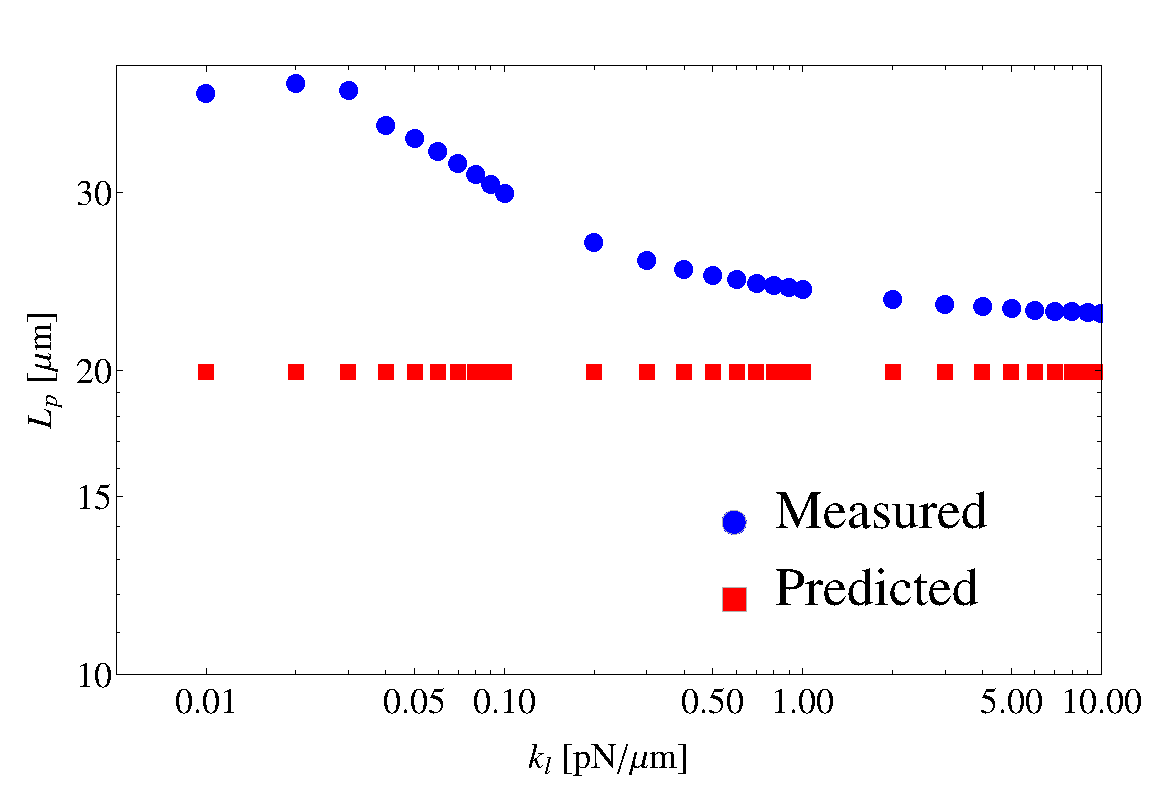
\includegraphics[width=\textwidth]{figs/figure2/kl_vs_lp_fit30.eps}
    \caption{\label{fig:kl}}
  \end{subfigure}%
  ~
  \begin{subfigure}{0.6\textwidth}
    \centering
    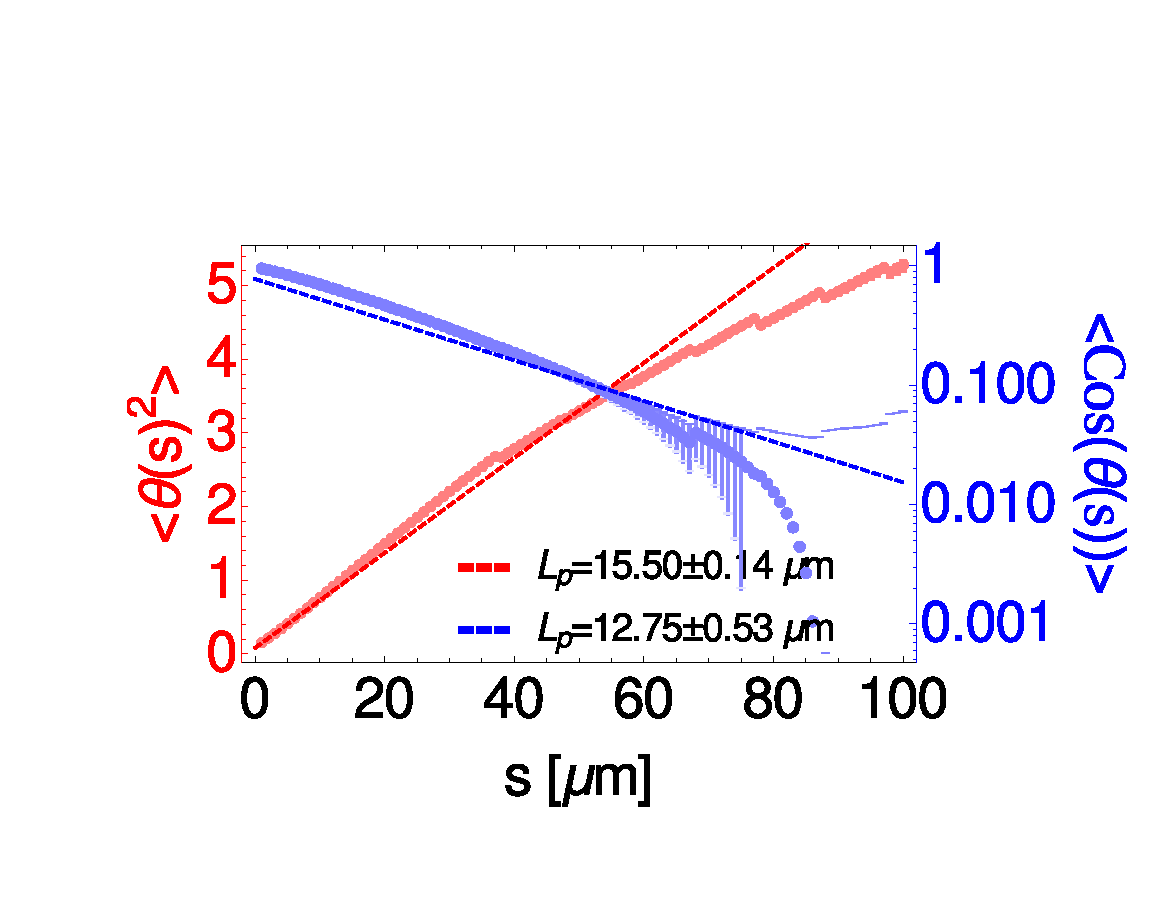
\includegraphics[width=\textwidth]{figs/figure2/sAvgd_L1-100.eps}
    \caption{\label{fig:lp_vs_l}}
  \end{subfigure}
  ~
  \begin{subfigure}{0.4\textwidth}
    \centering
    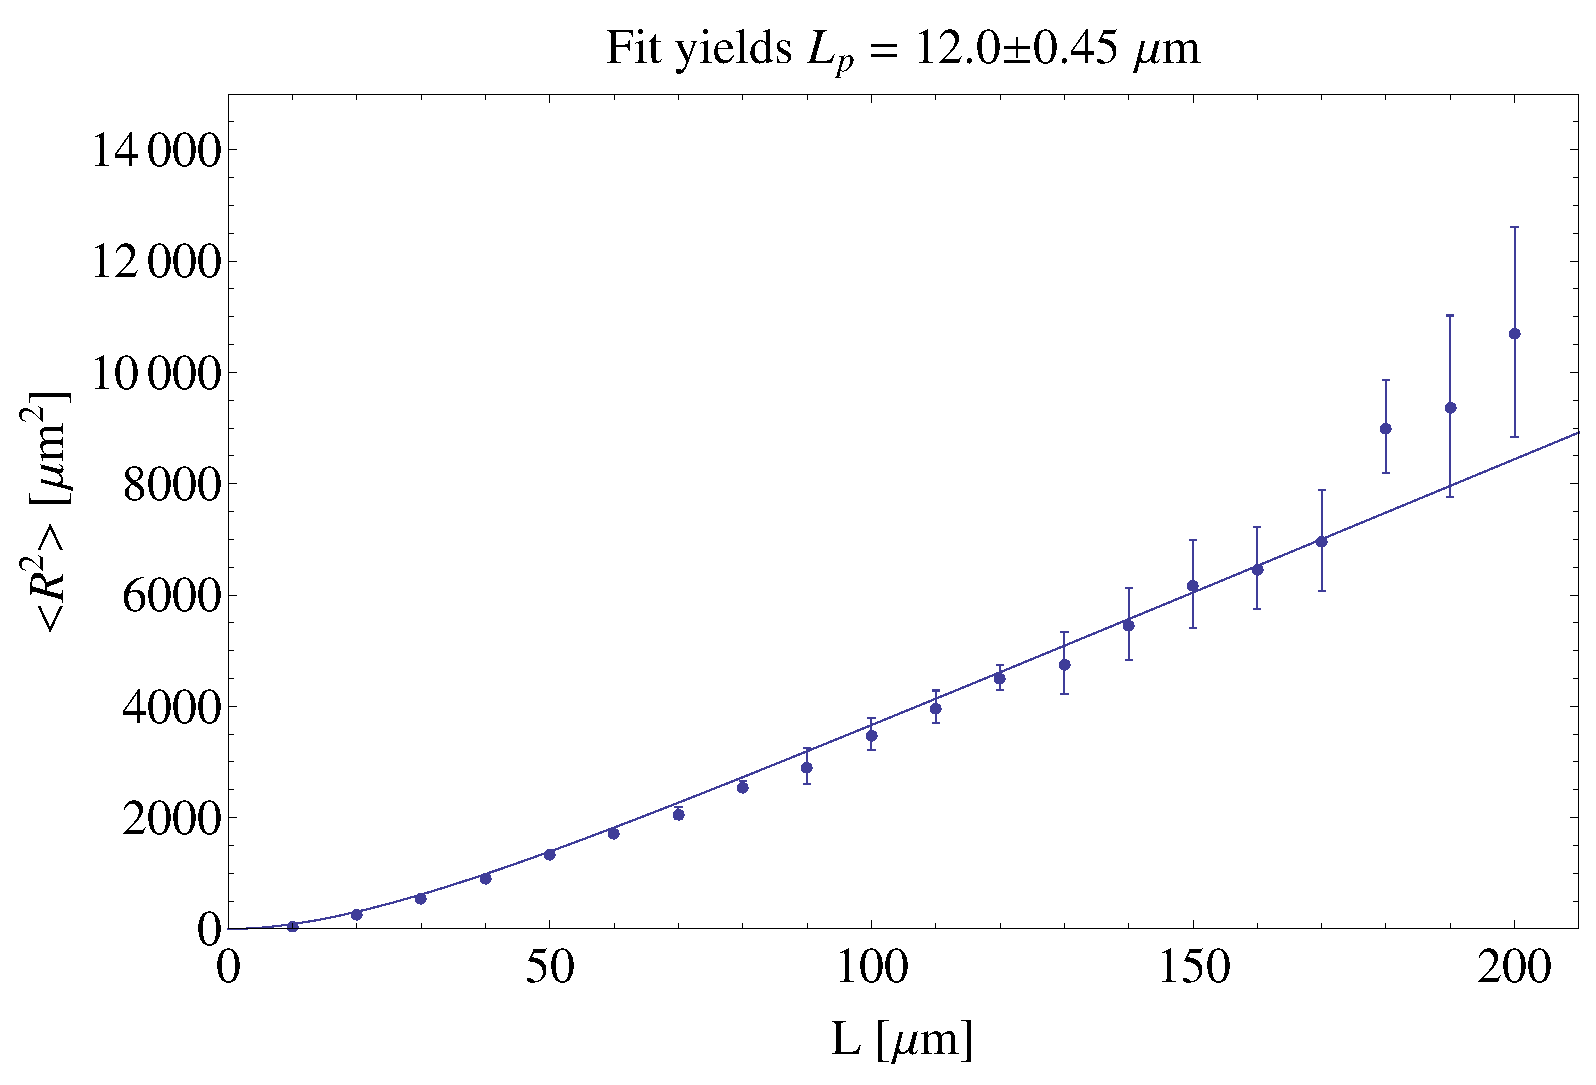
\includegraphics[width=\textwidth]{figs/figure2/R2vsL.eps}
    \caption{\label{fig:R2}}
  \end{subfigure}
  \label{fig:wlc_supp}
  \caption{
    \subref{fig:kl}Persistence length as function of stretching stiffness approaches correct answer for high
  enough stiffness. 
  \subref{fig:lp_vs_l}Methods $1$ and $2$ of measuring persistence length, described in main text using different length
  filaments.
  \subref{fig:R2} A third method for measuring persistence length, as function of end to end distance, described above.
}
\end{figure}
\subsection{Strain Stiffening} \label{strain_supp} 
\begin{figure}[H] 
  \begin{subfigure}{0.35\textwidth}
    \centering
    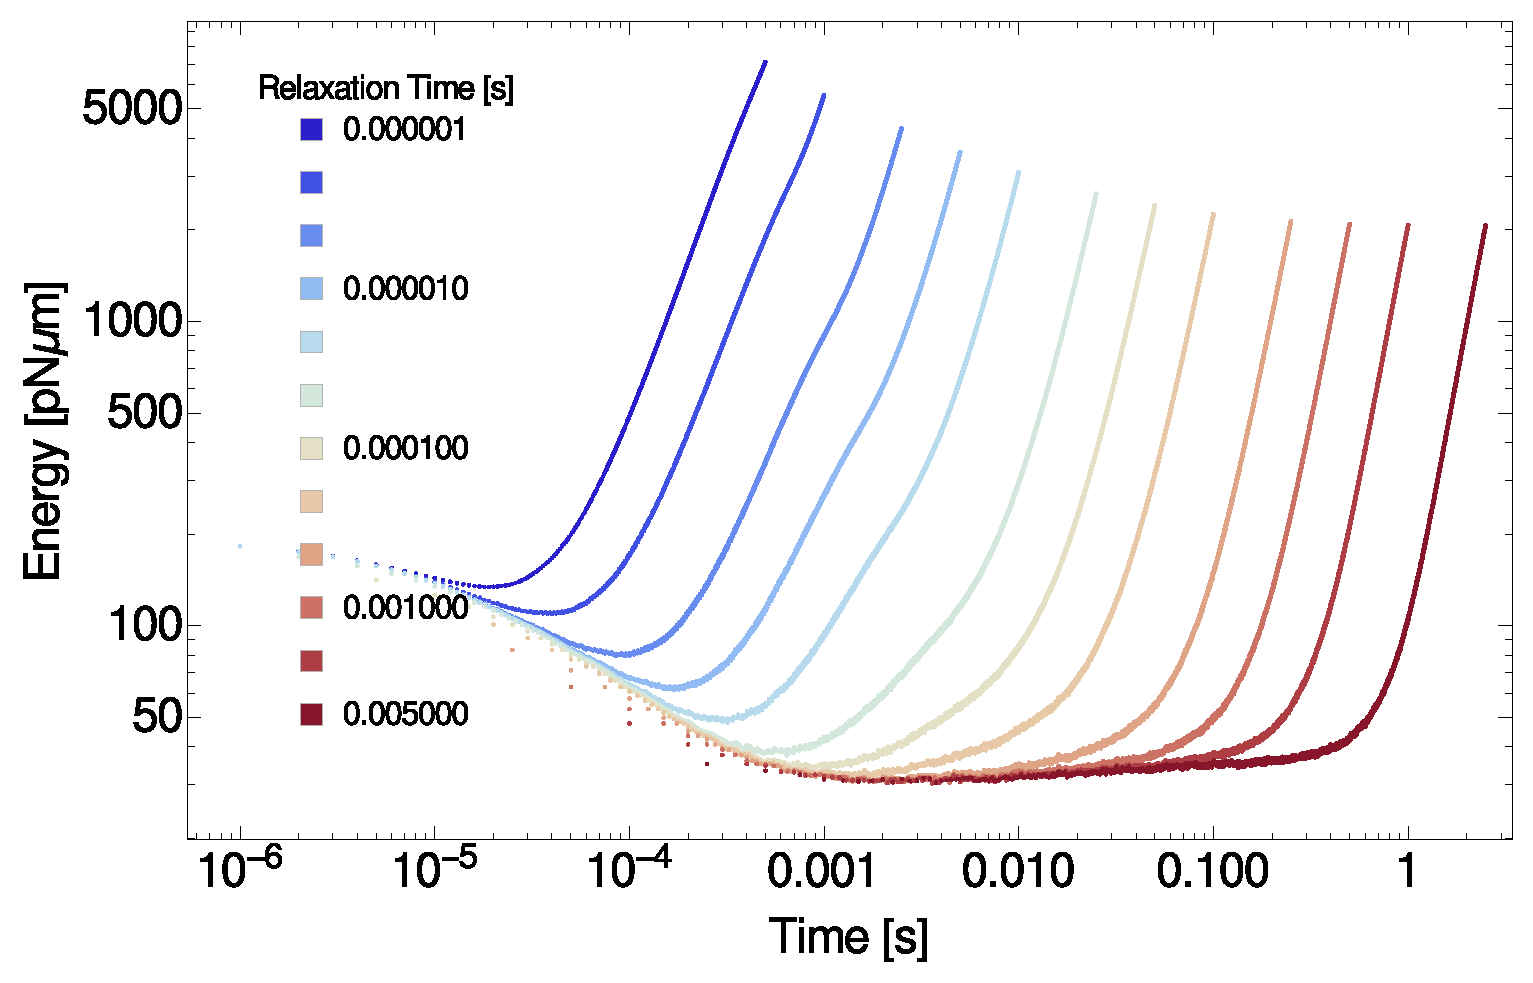
\includegraphics[width=\textwidth]{figs/elasticity/eng_vs_t_k100.eps}
    \caption{\label{fig:tRelax100}}
  \end{subfigure}
  \label{fig:tRelax}
  \caption{\subref{fig:tRelax10} Strain energy as function of time for various relax times $t_{relax}$ for stiff ($k_{cl}=100pN/\mu m$)
crosslinked networks}.
\end{figure}
\end{document}
